% SSEE — Paper 2: Bayesian MCMC Validation
% Compile: pdflatex (×2)
\documentclass[12pt,a4paper]{article}

\usepackage{amsmath,amssymb,amsfonts}
\usepackage{graphicx}
\graphicspath{{../results/figures/}}
\usepackage{booktabs}
\usepackage[colorlinks=true,linkcolor=red!70!black,citecolor=green!50!black,urlcolor=blue!80!black]{hyperref}
\usepackage{xcolor}
\usepackage{geometry}
\usepackage{natbib}
\usepackage{caption}
\usepackage{float}
\usepackage{array}

\geometry{margin=2.5cm}

\newcommand{\SSEE}{\ifmmode\mathrm{SSEE}\else\textsc{ssee}\fi}
\newcommand{\LCDM}{\ifmmode\Lambda\mathrm{CDM}\else$\Lambda$CDM\fi}
\newcommand{\KALz}{\mathrm{KAL}_0}
\newcommand{\kal}{\mathrm{KAL}}
\newcommand{\wz}{w_0}
\newcommand{\wa}{w_a}
\newcommand{\OmDE}{\Omega_{\mathrm{DE}}}
\newcommand{\Mssee}{M_{\mathrm{SSEE}}}
\newcommand{\Migimf}{M^{\mathrm{IGIMF}}_{\mathrm{bar}}}
\newcommand{\Mobs}{M^{\mathrm{obs}}_{\mathrm{dyn}}}
\newcommand{\AURA}{\mathcal{A}}
\newcommand{\DUAL}{\mathcal{D}}
\newcommand{\rdSSEE}{r_{d,\mathrm{SSEE}}}
\newcommand{\rdeff}{r_{d,\mathrm{eff}}}
\newcommand{\MIRA}{\ifmmode\mathcal{M}\else$\mathcal{M}$\fi}

\title{\textbf{Bayesian MCMC Validation of the Structural\\
Self-Energy Expansion Framework (SSEE)}:\\[6pt]
\large Model Comparison against $\Lambda$CDM and CPL\\
using DESI~DR2, Planck~2018, and Galaxy-Cluster Mass Data}

\author{Mike Edison Almeida Vallejo \\
\small \textit{Independent Researcher} \\
\small \href{mailto:mike.almeida1721@gmail.com}{mike.almeida1721@gmail.com} \\
\small ORCID: \href{https://orcid.org/0009-0008-2195-7836}{0009-0008-2195-7836}
}
\date{April 2026}

% Posterior H0 del MCMC reframe (prior H_glob=67.962±0.968, DESI DR2, geometría total 0.308881).
% 66.41 SUPERSEDED (V-L4-DESI 2026-07-09): el sector 0.160 estaba en E(z); con la
% materia total el posterior subia a 67.79 (0.50sigma del anchor; superado). 67.16 era DR1.
% CORREGIDO 2026-08-07: el 67.95/0.04sigma previo congelaba Om=0.308881 dentro de
% E(z), asi que el modelo solo se evaluaba fielmente en H0=67.962 (el ancla) y el
% posterior quedaba sesgado hacia ella (fix R25, 2026-07-25). Ese 67.79 quedo superado; el vigente sale de \val{h0_p2}.
% ACTUALIZADO 2026-09-29: prior H_glob = SH0ES·(1−f_screen) = 67.962 ± 0.968 (era el número puro
% con el σ de Planck 0.54) y r_d/distancias por CAMB. Valor vigente: \val{h0_p2} de results/logs/mcmc_paper2_reframe.json (semilla fija, 2026-10-01).
% Fuente: results/logs/mcmc_paper2_reframe.json (100w×25k, N_eff=79056) · distancias: h0_distancias_hglob.json.
\newcommand{\HZeroPosterior}{\val{h0_p2}^{+\val{h0_p2_mas}}_{-\val{h0_p2_menos}}}

\sloppy
% ACTA-PROCEDENCIA {"commit": "5651fc97a90dc17d52be0317b46142db9ac86fcb", "reproducible_desde_commit": true, "cambios_sin_commitear": [], "script": "src/valores_tex.py", "script_sha256": "cb5ceb2369bdef5e586d471d57d44a11a9fed354be540a96ce34da85e582efa4", "nucleo_sha256": "5cec8af72d88f154116c5a532e42a9b6ff7a5b4c3d86bcc6921eabb246698993", "entradas": {"manuscript/valores.yaml": "5fa01e91dd68164243d664a73264bb6c87431d2ec0bd69db87c62a983a55992d", "results/logs/kids_publicados.json": "6c25c98059ce91038215358b4e7ac9cfb40198f410354937cee4ea00b46654ff", "results/logs/p10_uv_fscreen.json": "8fb68b295c848e0292e5701e7de795ba7c7ba25e3292d776260bb3dea8970c95", "results/logs/s8_desde_b1.json": "6d225f4403fbfbe6934d7edca26aaefbbe19e05ef6c7b7eda842a259e798b1c1"}, "argv": ["src/valores_tex.py"], "fecha": "2026-09-30T19:35:24", "host": "mike-System-Product-Name", "python": "3.12.3", "versiones": {}, "nucleos": {"OMP_NUM_THREADS": null, "MKL_NUM_THREADS": null, "OPENBLAS_NUM_THREADS": null, "OMPI_COMM_WORLD_SIZE": null}}
% GENERADO por src/valores_tex.py desde manuscript/valores.yaml — NO EDITAR A MANO.
% Cada numero sale de un log de la cadena de procedencia (dvc.yaml + acta).
\providecommand{\val}[1]{\csname ssee@val@#1\endcsname}
\expandafter\def\csname ssee@val@H0_glob\endcsname{67.962142}  % results/logs/p10_uv_fscreen.json#H0_glob
\expandafter\def\csname ssee@val@PTE_k1000_lcdm\endcsname{0.010}  % results/logs/kids_publicados.json#PTE.lcdm.PTE
\expandafter\def\csname ssee@val@PTE_k1000_ssee\endcsname{0.012}  % results/logs/kids_publicados.json#PTE.ssee.PTE
\expandafter\def\csname ssee@val@S8_b1_lcdm\endcsname{0.8229}  % results/logs/s8_desde_b1.json#filas.LCDM.S8
\expandafter\def\csname ssee@val@S8_b1_lcdm_sigma\endcsname{0.0059}  % results/logs/s8_desde_b1.json#filas.LCDM.S8_sigma
\expandafter\def\csname ssee@val@S8_b1_ssee\endcsname{0.8261}  % results/logs/s8_desde_b1.json#filas.SSEE.S8
\expandafter\def\csname ssee@val@S8_b1_ssee_sigma\endcsname{0.0054}  % results/logs/s8_desde_b1.json#filas.SSEE.S8_sigma
\expandafter\def\csname ssee@val@S8_legacy_dato\endcsname{0.8265}  % results/logs/kids_publicados.json#kids_legacy.S8
\expandafter\def\csname ssee@val@S8_legacy_dato_sigma\endcsname{0.0176}  % results/logs/kids_publicados.json#kids_legacy.S8_sigma
\expandafter\def\csname ssee@val@chi2_k1000_lcdm\endcsname{262.75}  % results/logs/kids_publicados.json#PTE.lcdm.chi2
\expandafter\def\csname ssee@val@chi2_k1000_publicado\endcsname{260.31}  % results/logs/kids_publicados.json#kids1000_maxpost.chi2
\expandafter\def\csname ssee@val@chi2_k1000_ssee\endcsname{265.44}  % results/logs/kids_publicados.json#PTE.ssee.chi2
\expandafter\def\csname ssee@val@dAIC_k1000\endcsname{-5.31}  % results/logs/kids_publicados.json#seleccion_kids1000.delta_AIC
\expandafter\def\csname ssee@val@dBIC_k1000\endcsname{-19.0}  % results/logs/kids_publicados.json#seleccion_kids1000.delta_BIC
\expandafter\def\csname ssee@val@dchi2_k1000\endcsname{2.69}  % results/logs/kids_publicados.json#seleccion_kids1000.delta_chi2
\expandafter\def\csname ssee@val@fscreen_IR\endcsname{0.067253}  % results/logs/p10_uv_fscreen.json#f_screen_IR
\expandafter\def\csname ssee@val@fscreen_UV_corr\endcsname{0.002268}  % results/logs/p10_uv_fscreen.json#f_screen_UV_corr
\expandafter\def\csname ssee@val@fscreen_full\endcsname{0.069522}  % results/logs/p10_uv_fscreen.json#f_screen_full
\expandafter\def\csname ssee@val@logA_b1_lcdm\endcsname{3.045}  % results/logs/s8_desde_b1.json#filas.LCDM.logA
\expandafter\def\csname ssee@val@logA_b1_ssee\endcsname{3.042}  % results/logs/s8_desde_b1.json#filas.SSEE.logA
\expandafter\def\csname ssee@val@logA_b1_ssee_sigma\endcsname{0.013}  % results/logs/s8_desde_b1.json#filas.SSEE.logA_sigma
\expandafter\def\csname ssee@val@p_dchi2_k1000\endcsname{0.61}  % results/logs/kids_publicados.json#seleccion_kids1000.p_delta_chi2
\expandafter\def\csname ssee@val@sK_IR\endcsname{0.403302}  % results/logs/p10_uv_fscreen.json#s_K_IR
\expandafter\def\csname ssee@val@sK_UV_corr\endcsname{0.013603}  % results/logs/p10_uv_fscreen.json#s_K_UV_corr
\expandafter\def\csname ssee@val@sK_full\endcsname{0.416905}  % results/logs/p10_uv_fscreen.json#s_K_full
\expandafter\def\csname ssee@val@tension_b1_lcdm\endcsname{2.59}  % results/logs/s8_desde_b1.json#filas.LCDM.tension_kids
\expandafter\def\csname ssee@val@tension_b1_ssee\endcsname{2.73}  % results/logs/s8_desde_b1.json#filas.SSEE.tension_kids
\expandafter\def\csname ssee@val@z_k1000_lcdm\endcsname{2.5}  % results/logs/kids_publicados.json#PTE.lcdm.z
\expandafter\def\csname ssee@val@z_k1000_ssee\endcsname{2.4}  % results/logs/kids_publicados.json#PTE.ssee.z

\begin{document}
\maketitle

\begin{abstract}
We present a Bayesian validation of the dynamical sector of the
Structural Self-Energy Expansion (\SSEE) framework
\citep{SSEE_paperI} against DESI~DR2 baryon acoustic oscillation data
\citep{DESI_DR2} and a compressed Planck~2018 prior \citep{Planck2018}, with
galaxy-cluster dynamical masses \citep{Zhang2026} as a separate consistency test. Using geometric constants fixed algebraically
by $\pi$ and the golden ratio $\varphi$ — with $H_0$ and $\Omega_b h^2$ as the only
sampled parameters — we compare the model against \LCDM\ and a free CPL
parameterisation via posterior constraints, information criteria, and
predictive checks, using \textsc{emcee} \citep{emcee,GoodmanWeare2010} with $N_{\rm walkers}=100$,
$N_{\rm steps}=25{,}000$ ($2.5\times10^6$ total evaluations), and a same-bin correlated block-diagonal covariance approximation for the DESI~DR2 BAO measurements; convergence
diagnostics (including $N_{\rm eff}=4{,}402$ effective samples for \SSEE) are
reported in Table~\ref{tab:convergence}.
The \SSEE\ prediction $(\wz,\wa)=(-0.840,-0.670)$, fixed algebraically by the
closed dictionary \citep{AlmeidaSSEE2026genesis} and not fitted to the data,
lies within $0.24\sigma$ of the official DESI~DR2 $w_0w_a$CDM posterior
(DESI+CMB+Pantheon+; arXiv:2503.14738, eq.~26) in the $\wz$--$\wa$ plane, and
within $1.2$--$1.5\sigma$ of the DESY5/Union3/no-SN combinations
(a parameter-free postdiction).
The $H_0$ posterior is $\HZeroPosterior$~km\,s$^{-1}$\,Mpc$^{-1}$,
obtained with the global rate of the screening cascade as the $H_0$ prior
($H_0^{\rm glob}=H_{\rm SH0ES}(1-f_{\rm screen})=\val{H0_GLOBAL_d3}\pm0.968$; Papers~3, 9--10, \S\ref{sec:prior_mira}),
$\val{h0_p2_dhglob}\sigma$ from that prediction.
Against all $\val{clz_rgimf_N}$ cluster dynamical masses of \citet{Zhang2026}, the
\SSEE\ matter content in general relativity, $M_{\rm dyn}=(\omega_m/\omega_b)\,M_{\rm bar}$
with no free parameter, is consistent at $\val{clz_rgig_sig}\sigma$ with the IGIMF
baryon baseline --- as is \LCDM\ ($\val{clz_lcig_sig}\sigma$): clusters test the matter
content but do not discriminate between the two backgrounds.
With $(w_0,w_a)$ fixed algebraically and one free parameter $H_0$, SSEE is
favoured by $\Delta\mathrm{BIC}=\val{p2_dBIC_lcdm}$ over \LCDM\ and $\val{p2_dBIC_cpl}$ over CPL, and
predicts the DESI~DR2 test set better in leave-one-out cross-validation ---
so the $\wz$--$\wa$ prediction is genuinely preferred by current BAO data.
The background geometry uses the \emph{total} gravitating matter density
$\Omega_m=\omega_m/h^2=\val{OMEGA_M_TOTAL_d6}$ ($\omega_m$-direct; no matter factor, OP-8
dissolved), for which the SSEE sound horizon matches \LCDM\
($r_d^{\SSEE}/r_d^{\LCDM}=1.002$) and $\Omega_m$ agrees with Planck at
$0.88\sigma$. The saturation $s_m=1+w_0=\val{S_M_d6}$ is a number of the
dark-energy equation of state, not a density, and does not enter the
background geometry.
\end{abstract}

% Cross-reference note for reviewers
\noindent\textbf{Note on the background matter density:} Throughout, the
background geometry ($E(z)$, the sound horizon $r_d$, and all BAO distances)
uses the \emph{total} gravitating matter density $\Omega_m=\omega_m/h^2=\val{OMEGA_M_TOTAL_d6}$,
built piece-by-piece from SSEE algebra ($\omega_m$-direct; no matter factor,
OP-8 dissolved; Paper~3). The saturation $s_m=1+w_0=\val{S_M_d6}$ is a number of
the dark-energy equation of state, \emph{not} a matter density, and never enters
$E(z)$. With the total density the SSEE sound horizon matches
$\Lambda$CDM and model selection yields a single, unambiguous figure:
$\Delta\mathrm{BIC}=\val{p2_dBIC_lcdm}$ favouring SSEE over $\Lambda$CDM and $\val{p2_dBIC_cpl}$ over CPL
(Section~\ref{sec:bic}).


\clearpage
{\small\tableofcontents}
\clearpage

\section{Introduction}
\label{sec:intro}

The discovery of cosmic acceleration \citep{Perlmutter1999,Riess1998} has motivated
a broad class of dark energy models, from the cosmological constant to dynamical
scalar fields \citep{Weinberg2013,Clifton2012}.
Baryon acoustic oscillations, first detected in galaxy surveys by \citet{Eisenstein2005},
have since become a primary geometric probe of the expansion history.
The \SSEE\ framework \citep{SSEE_paperI} is a
\textbf{minimal-parameter phenomenological framework} that encodes the
cosmological background as algebraic combinations of $\pi$ and
$\varphi=(1+\sqrt{5})/2$.
The background sector $(w_0,w_a,\Omega_{\rm DE},\Omega_m)$ tested in this
paper carries zero dimensionless fitted parameters, and no WIMP, QCD-axion, or SUSY
dark-matter particle is introduced; phenomenological extensions in the dark-matter
sector (Paper~6) introduce ans\"atze tracked as open problems
(see Paper~1, \S1.3, and \texttt{OPEN\_PROBLEMS.md}).
Paper~1, Appendix~A provides a complete Lagrangian (k-essence + Israel--Stewart
viscosity) derived algebraically from $\{\varphi,\pi\}$, with zero free parameters
at the EFT background level.
Its current operational status is that of a
\emph{predictive phenomenology} — one whose central predictions are
fixed before confronting data.
Paper~I established theoretical foundations and demonstrated qualitative
alignment with DESI~DR2 dynamical dark-energy trends \citep{DESI_DR2}
and galaxy-cluster mass data \citep{Zhang2026}, but performed no formal
statistical inference.

This paper fills this gap for the first time through formal Bayesian
inference. Following the methodology recommended by contemporary
dynamical dark-energy analyses \citep{DESI_DR2,Moresco2017}, we conduct a
full Bayesian MCMC evaluation with four aims:
\begin{enumerate}
  \item Quantify whether \SSEE\ remains competitive under formal
    Bayesian inference against \LCDM\ and free CPL alternatives.
  \item Test, symmetrically against \LCDM, whether galaxy-cluster dynamical
    masses are consistent with the \SSEE\ matter content.
  \item Document why the naive $\OmDE^{\SSEE}\approx0.840$ vs
    $\Omega_\Lambda\approx0.685$ comparison is a category error
    ($s_{\rm DE}$ vs.\ density fraction) and localise its origin in the
    retired two-sector framing (see \S\ref{sec:folding}).
  \item Provide a roadmap for the modified Friedmann CMB analysis
    and semi-linear transfer function required in Paper~3.
\end{enumerate}

The framing is explicit: \textit{the goal of this paper is to test the
ansatz against current data, not to defend it}. Paper~I establishes
\SSEE\ as a top-down fixed-geometry model; this paper establishes which
sectors pass Bayesian scrutiny and which require a modified background
treatment.

\section{SSEE Model Summary}
\label{sec:model}

\subsection{Algebraic constants}

From $\pi$ and $\varphi=(1+\sqrt{5})/2$, the framework defines the
structural retention $\KALz$ and the CPL \citep{Chevallier2001,Linder2003} parameters as:
\begin{align}
  \KALz &= \frac{\pi+\varphi}{2}+\pi \approx \val{KAL0_d4}, \label{eq:kal0} \\
  \wz^{\SSEE} &= -\frac{T_r}{M_v}\approx-0.840, \quad
  \wa^{\SSEE} = -\frac{P_{sc}}{I_g}\approx-0.670.
  \label{eq:ssee_pars}
\end{align}
All three quantities are fixed by geometry; no fitting is performed.
Note that $\wz+\wa=-1.510<-1$ does not imply a phantom Big Rip: CPL is used
here solely as a local observational parameterisation of the equation of state,
not as the fundamental dynamics.  In the \SSEE\ framework, the dark-energy
density saturates at the finite $T_r/M_v$ boundary of the action at
$a\to\infty$, guaranteeing universal stability; see Paper~1 \S3.4
\citep{SSEE_paperI} for the full stability argument.
The equation-of-state-sector saturation quantity is similarly fixed:
$s_{\rm DE}^{\SSEE}=T_r/M_v\approx0.840$ (not a density fraction), with the
algebraic matter-sector complement
\begin{equation}
  s_m = 1-s_{\rm DE}^{\SSEE} \approx 0.160.
  \label{eq:om_eff}
\end{equation}
The fixed-geometry model is effectively parameter-free at the geometric
level; only $H_0$ and $\Omega_b h^2$ are inferred from data.

\subsection{Friedmann background ($\omega_m$-direct)}

\begin{equation}
  H^2(z) = H_0^2\!\left[\Omega_m(1+z)^3
  + \Omega_{\rm DE}\,f_{\rm DE}(z)\right],
  \label{eq:Hssee}
\end{equation}
where $f_{\rm DE}(z)=(1+z)^{3(1+\wz+\wa)}\exp[-3\wa z/(1+z)]$ is the
standard CPL dark-energy evolution, here used solely to translate the
fixed \SSEE\ geometric parameters into observable distances.
There is one matter density, $\Omega_m=\omega_m/h^2=\val{OMEGA_M_TOTAL_d6}$
(\S\ref{sec:folding}; no matter factor, OP-8 dissolved), hence
$\Omega_{\rm DE}=1-\Omega_m=\val{OMDE_DENS_d6}$.
The only sampled cosmological parameter is $H_0$; the algebraic
quantities ($\wz,\wa,s_{\rm DE}^{\SSEE},\KALz$) are fixed by geometry
as described in Section~\ref{sec:model}. The equation-of-state-sector
quantities $s_{\rm DE}^{\SSEE}=T_r/M_v\approx0.840$ and
$s_m=1-s_{\rm DE}^{\SSEE}\approx0.160$ do not enter the background
densities (see \S\ref{sec:folding}).

\begin{figure}[H]
  \centering
  \includegraphics[width=0.82\textwidth]{fig3_omega_de.pdf}
  \caption{\textit{Left}: $s_{\rm DE}^{\SSEE}=T_r/M_v\approx0.840$ (red line),
  the equation-of-state-sector saturation quantity (not a density fraction;
  the physical density is $\Omega_{\rm DE}=\val{OMDE_DENS_d6}$), shown against
  Planck~2018 $\Omega_\Lambda\approx0.685$ (blue) and
  DESI~DR2 $1\sigma$/$2\sigma$ bands for scale. \textit{Right}: Structural context
  showing the algebraic origin of $s_{\rm DE}$ from the $\pi$--$\varphi$ invariants.}
  \label{fig:omega_de}
\end{figure}

\subsection{Cluster mass formula}

\SSEE\ does not modify gravity: its effective-field-theory functions are
$\alpha_T=\alpha_M=\alpha_B=0$ (Paper~7), so gravitational waves travel at the
speed of light and the effective gravitational coupling is Newton's ($\mu=1$,
Paper~8). A virialised cluster therefore weighs its whole matter content, as in
\LCDM, and the dynamical mass follows from the baryonic one by the cosmic
matter-to-baryon ratio of the model:
\begin{equation}
  \Mssee = \frac{\omega_m}{\omega_b}\,M_{\rm bar}
  = \Bigl(1+\mathrm{KAL_0}\,n_s+\frac{\omega_\nu}{\omega_b}\Bigr)M_{\rm bar}
  = (1+\val{clz_cdm}+\val{clz_nu})\,M_{\rm bar}=\val{clz_K_rg}\,M_{\rm bar},
  \label{eq:Mcluster}
\end{equation}
where the second form uses the forward identity $\omega_c=\mathrm{KAL_0}\,\omega_b\,n_s$
(Paper~1). There is no free parameter. The \LCDM\ control uses its own ratio,
$\Omega_m/\Omega_b=\val{clz_K_lcdm}$ from Planck~2018.
An earlier version of this analysis used
$M=M_{\rm bar}\,\mathrm{KAL_0}\,(1+f_\nu)$ with $f_\nu=0.020$; that form belonged
to a modified-gravity reading of the framework (the ``MOND-like'' limit of
Paper~8, which the cluster lens A1689 excludes) and is withdrawn, together with
$f_\nu$: computed as the paper declared it --- relic neutrinos bound to a cluster
--- that fraction is below $10^{-5}$.%
% ORIGEN: f_nu <= 2e-6 (techo Tremaine-Gunn), results/logs/fnu_tremaine_gunn.json

\subsection{The sound horizon under the $\omega_m$-direct reframe}
\label{sec:folding}

Placing the cold sector alone ($1+w_0=\val{S_M_d6}$) in the background geometry would
give a drag scale $\rdSSEE \approx 175.6$\,Mpc, far from the Planck-inferred
$r_d=147.09\pm0.26$\,Mpc \citep{Planck2018}. That figure is a category error:
$0.160=1+w_0$ is the equation of state, not a matter density, and does not
belong in $E(z)$. The physical sound horizon is set by the CMB-sector matter
density, with \emph{no} $|w_0|$ rescaling. The recombination matter budget is the standard physical
$\omega_m=\omega_b+\omega_c+\omega_\nu=\val{OMEGA_M_H2_d5}$, built piece-by-piece from
SSEE algebra ($\omega_c=\mathrm{KAL_0}\,\omega_b\,n_s$, forward; Paper~3), so
that $\Omega_{m,\mathrm{CMB}}=\omega_m/h^2=\val{OMEGA_M_TOTAL_d6}$ and a CAMB integration of
the recombination physics gives
\begin{equation}
  r_d^{\,\omega_m\text{-direct}} = 147.17\;\text{Mpc}
  \quad (0.32\sigma\ \text{from Planck; Paper~3}),
  \label{eq:rd_mapping}
\end{equation}
with \emph{no} matter factor.
The earlier post-hoc mapping $\rdSSEE\times|w_0|\approx147.5$\,Mpc, and the
structural ratio $\Omega_{m,\mathrm{CMB}}/\Omega_{m,\mathrm{dyn}}\approx
\mathrm{MIRA}\approx1.999$, are \emph{superseded} by this direct construction
(OP-8 dissolved; the actual ratio is $\val{OMEGA_M_TOTAL_d6}/0.160=1.93$, not a fixed factor).
MIRA survives only as the Hubble screening amplitude of Paper~9.
There is one matter density, $\Omega_m=\omega_m/h^2=\val{OMEGA_M_TOTAL_d6}$; the quantity
formerly written $\Omega_{m,\rm dyn}=\val{S_M_d6}$ is $1+w_0$, an equation-of-state
parameter, and never was a density (Paper~1, \S1.4;
the $\phi$-DM sector that once separated them is retracted in Paper~6).
The falsifiable content therefore moves from the $|w_0|$ coincidence to the
direct CMB fit of Paper~3 (canonical $\Delta\mathrm{BIC}=\val{b1_dBIC}$ full \texttt{plik}
MCMC; $-26.03$ \texttt{plik\_lite} TTTEEE+low-$\ell$ point estimate): if that fit had yielded $\chi^2_r\gg1$ or excluded
$r_d^{\,\omega_m\text{-direct}}$, the construction would be falsified.

%% 2026-10-01: retirada la figura de la interpolacion KAL(x) Newton-MOND (fig4_KAL_interpolation):
%% describia la lectura de gravedad modificada que el modelo vigente (alpha_T=alpha_M=alpha_B=0) no usa.

\section{Datasets and Likelihoods}
\label{sec:data}

\subsection{DESI DR2 BAO}

We use 13 BAO measurements from DESI~DR2 \citep{DESI_DR2} at
$0.295\leq z\leq2.330$ (Table~\ref{tab:bao_data}). These 13 data points
span five tracer populations across $0.3\lesssim z\lesssim 2.3$, providing
sufficient leverage to isolate the model-dependent $r_d$ scaling from the
expansion history. The BAO log-likelihood uses a block-diagonal covariance incorporating the same-tracer correlation between $D_M$ and $D_H$ (coefficients $r_{MH}$ taken directly from Table~4 of \citealt{DESI_DR2}), which is the dominant off-diagonal term ($|r_{MH}|$ up to $\sim0.4$).\footnote{Cross-tracer (inter-redshift) covariances are not propagated. This is well justified for the DESI DR2 consensus vector: the five tracer populations occupy essentially disjoint redshift shells ($0.3\lesssim z\lesssim 2.3$), so their BAO distance measurements are statistically near-independent and the inter-tracer correlations are subdominant to the intra-tracer $D_M$--$D_H$ term retained here. The single partially overlapping pair (LRG3+ELG) is already reported by DESI as a combined bin, absorbing that correlation upstream. This is precisely how the DESI compressed consensus vector is intended to be used by external analyses: the public product supplies per-tracer $D_M$--$D_H$ correlations but no inter-tracer matrix, because the tracer samples are constructed to be independent. Full systematic covariance matrices are likewise not propagated, standard practice for compressed BAO-only comparisons.}
\begin{equation}
  \ln\mathcal{L}_{\rm BAO}
  = -\tfrac{1}{2} (\mathbf{q}^{\rm pred}-\mathbf{q}^{\rm obs})^\top \mathbf{C}^{-1} (\mathbf{q}^{\rm pred}-\mathbf{q}^{\rm obs}),
\end{equation}
with the sound horizon from a power-law expansion about the Planck~2018
point \citep{Planck2018}, used here as an auxiliary approximation for model
comparison. Its exponents are the local logarithmic derivatives of the
\citet{EisensteinHu1998} fitting formula at that point, and its normalization
is the Boltzmann value there (compare the global fit of
\citealt{Aubourg2015}):
\begin{equation}
  r_d = 147.27\!\left(\frac{\Omega_m h^2}{0.1432}\right)^{\!-0.255}\!
  \left(\frac{\Omega_b h^2}{0.02237}\right)^{\!-0.134}\!\text{Mpc}.
  \label{eq:rd}
\end{equation}

\begin{table}[H]
\centering
\caption{DESI DR2 BAO measurements \citep{DESI_DR2}.}
\label{tab:bao_data}
\small
\begin{tabular}{lllrr}
\toprule
$z_{\rm eff}$ & Tracer & Quantity & Value & $\sigma$ \\
\midrule
0.295 & BGS         & $D_V/r_d$  &  7.942 & 0.075 \\
0.510 & LRG1        & $D_M/r_d$  & 13.588 & 0.167 \\
0.510 & LRG1        & $D_H/r_d$  & 21.863 & 0.425 \\
0.706 & LRG2        & $D_M/r_d$  & 17.351 & 0.177 \\
0.706 & LRG2        & $D_H/r_d$  & 19.455 & 0.330 \\
0.934 & LRG3+ELG1   & $D_M/r_d$  & 21.576 & 0.152 \\
0.934 & LRG3+ELG1   & $D_H/r_d$  & 17.641 & 0.193 \\
1.321 & ELG2        & $D_M/r_d$  & 27.601 & 0.318 \\
1.321 & ELG2        & $D_H/r_d$  & 14.176 & 0.221 \\
1.484 & QSO         & $D_M/r_d$  & 30.512 & 0.760 \\
1.484 & QSO         & $D_H/r_d$  & 12.817 & 0.516 \\
2.330 & Ly$\alpha$  & $D_M/r_d$  & 38.988 & 0.531 \\
2.330 & Ly$\alpha$  & $D_H/r_d$  &  8.632 & 0.101 \\
\bottomrule
\end{tabular}
\end{table}

\subsection{SSEE-self-consistent $H_0$ prior: the $\omega_m$-direct CMB anchor}
\label{sec:prior_mira}

To preserve methodological coherence between this BAO sector and the CMB
sector (Paper~3), the $H_0$ prior used here is not the published
$\Lambda$CDM-calibrated Planck~2018 value
($67.36\pm0.54$~km\,s$^{-1}$\,Mpc$^{-1}$, \citealt{Planck2018}),
but the $H_0$ that the Planck~\texttt{plik\_lite} TTTEEE likelihood itself
prefers under the SSEE background. With the baryon and cold-matter densities
fixed by SSEE algebra ($\omega_b=(\pi-\varphi)/[3(\varphi+\pi)^2]=\val{OMEGA_B_H2_d6}$,
$\omega_c=\mathrm{KAL_0}\,\omega_b\,n_s=\val{OMEGA_C_H2_d6}$; Paper~3, $\omega_m$-direct),
the CMB $\chi^2$ is minimised at the global rate returned by the SSEE
screening cascade (Papers~9--10), which takes the measured SH0ES rate as input:
\begin{equation}
  H_0^{\rm prior,SSEE} \;=\; H_0^{\rm glob} \;=\; H_{\rm SH0ES}\,(1-f_{\rm screen}) \;=\; \val{H0_GLOBAL_d3}\pm0.968 \;\text{km\,s}^{-1}\,\text{Mpc}^{-1},
  \label{eq:H0_prior_alg}
\end{equation}
where the uncertainty is the SH0ES error propagated through the (multiplicative)
screening factor, and the central value reproduces the dimensionless algebraic
target $3(\varphi+\pi)^2$ to $4.2\times10^{-6}$. The background
$H$ and the CMB anchor coincide --- they are not two numbers --- and the
matter density follows as $\Omega_{m,\mathrm{CMB}}=\omega_m/h^2=\val{OMEGA_M_TOTAL_d6}$,
with \emph{no} matter factor (the earlier MIRA mapping
$\Omega_{m,\mathrm{CMB}}=\mathrm{MIRA}\,\Omega_{m,\mathrm{dyn}}=0.31993$ is
superseded; OP-8 dissolved). Adopting this prior eliminates the otherwise unavoidable
cross-framework contamination introduced by using a $\Lambda$CDM-calibrated
constraint on the early Universe to fit a non-$\Lambda$CDM late-time
geometry. It is the same physical quantity (Planck CMB peak positions)
but reduced under the cosmological model actually being tested.

The only sampled parameters in the SSEE chain are $H_0$ and $\Omega_b h^2$.
The matter density is not sampled. The background geometry --- $E(z)$, the
sound horizon $r_d$, and every BAO distance --- uses the \emph{total} algebraic
matter density $\Omega_{m,\mathrm{CMB}}=\omega_m/h^2=\val{OMEGA_M_TOTAL_d6}$
(\S\ref{sec:folding}, \S\ref{sec:results_cosmo}); the value
$s_m=(\pi-\varphi)/[2(\varphi+\pi)]=1+w_0=\val{S_M_d6}$ is a saturation of the
equation of state, not a density, and does \emph{not} enter $E(z)$. Thus $r_d$ is computed from
$\omega_m = \Omega_{m,\mathrm{CMB}}(H_0/100)^2$ self-consistently.
A BBN prior $\Omega_b h^2 = 0.02218\pm0.00055$ \citep{Schoneberg2024} is adopted
for the baryon density, consistent with the SSEE algebraic value
$\Omega_b h^2 = (\pi-\varphi)/[3(\varphi+\pi)^2] = \val{OMEGA_B_H2_d6}$ (Paper~4)
at $0.4\sigma$.
Compared on the same footing --- total against total --- the SSEE matter
density agrees with the $\Lambda$CDM-Planck value
$\Omega_m = 0.3153\pm0.0073$ at $0.88\sigma$ ($\Omega_m=\val{OMEGA_M_TOTAL_d6}$).
A two-sector $\phi$-DM construction was previously invoked to describe how
this total partitions across scales; it is retracted in Paper~6, which finds a
single matter sector sufficient against raw shear data. The comparison above
uses the total density and is unaffected.

\subsection{Galaxy-cluster masses}

We use every system in Tables~II and~III of \citet{Zhang2026}:
$\val{clz_nII}$ WINGS clusters (with NGC\,5044) and $\val{clz_nIII}$ 2MASS clusters,
without selection. For each, the tables give the Newtonian dynamical mass
within the virial radius, $M_{\rm N,dyn}$, and the total baryonic mass under
two stellar initial mass functions: the canonical IMF and the integrated
galaxy-wide IMF (IGIMF), whose additional stellar remnants raise the baryonic
budget. Each predicted mass is compared with $M_{\rm N,dyn}$, with the
uncertainties of both masses added in quadrature (using the side of each
asymmetric error bar that faces the prediction, and a floor equal to the
rounding of the tables).

The cluster test is \emph{not} part of the MCMC likelihood. Neither model has a
free parameter in it, so it cannot move any posterior; it is reported
separately, in \S\ref{sec:results_clusters}, with \LCDM\ run through the
identical comparison.%
% 2026-10-01: la version anterior usaba Coma, A2029, A478 y el Bullet atribuidos a
% Zhang+2026; Coma y el Bullet no estan en sus tablas y A2029/A478 tenian otros
% numeros. Esa muestra y la de extension (masa barionica = f_b*M_obs, circular)
% quedan retiradas. Fuente unica: data/raw/zhang2026/tablas_II_III.tex (con sha).

\section{Bayesian Framework and Priors}
\label{sec:bayes}

\begin{table}[H]
\centering
\caption{Model parameterisations.}
\label{tab:models}
\begin{tabular}{llll}
\toprule
Model & Free parameters & Fixed & $k$ \\
\midrule
\SSEE & $H_0,\;\Omega_b h^2$ & $\wz,\wa,s_{\rm DE},\KALz$ (algebraic) & 2 \\
\LCDM      & $H_0,\;\Omega_m,\;\Omega_b h^2$ & $\wz=-1,\wa=0$ & 3 \\
CPL        & $H_0,\;\Omega_m,\;\wz,\;\wa,\;\Omega_b h^2$ & --- & 5 \\
\bottomrule
\end{tabular}
\end{table}

All models share a BBN prior $\Omega_b h^2\sim\mathcal{N}(0.02218,\,0.00055^2)$ \citep{Schoneberg2024}.
For \LCDM\ and CPL, the full 3D Planck prior is applied. For \SSEE,
the Planck prior reduces to a marginal Gaussian on $H_0$ only, since
$\Omega_m$ is fixed. CPL carries weakly informative priors
$\wz\sim\mathcal{N}(-1,0.5^2)$ and $\wa\sim\mathcal{N}(0,1^2)$.

Table~\ref{tab:param_hierarchy} classifies every quantity in the \SSEE\
MCMC by its structural role. The distinction between fixed-by-geometry,
sampled, and derived quantities is essential for interpreting the
information-criterion penalties in Section~\ref{sec:model_comparison}.
\SSEE\ samples only $H_0$ and $\Omega_b h^2$, while \LCDM\ and CPL
additionally sample $\Omega_m$ (and $\wz,\wa$ for CPL).

\begin{table}[H]
\centering
\caption{Parameter hierarchy in the \SSEE\ MCMC. Categories:
\textbf{Fixed by geometry} = algebraically determined, never sampled;
\textbf{Sampled} = inferred via MCMC; \textbf{Derived} = computed from
sampled values; \textbf{Mapped} = structural hypothesis (acoustic-scale mapping), to be validated in Paper~3.}
\label{tab:param_hierarchy}
\begin{tabular}{@{}lllp{4.2cm}@{}}
\toprule
Parameter & Category & Origin/Value & Notes \\
\midrule
$\wz,\,\wa$          & \textbf{Fixed by geometry} & Eqs.~\eqref{eq:ssee_pars} & $\pi,\varphi$ invariants; not fitted \\
$s_{\rm DE},\,\KALz$  & \textbf{Fixed by geometry} & $T_r/M_v;\ \beta+\pi$     & Algebraically closed \\
$H_0$                & \textbf{Sampled}           & $\mathcal{U}[60,80]$      & Only cosmological free parameter \\
$\Omega_b h^2$       & \textbf{Sampled}           & BBN prior                 & Shared with \LCDM, CPL \\
$r_d$                & \textbf{Derived}           & Friedmann background      & Eq.~\eqref{eq:rd}; carries background mismatch \\
$\rdeff$             & \textbf{Mapped (hypothesis)}& Acoustic-scale hypothesis & Eq.~\eqref{eq:rd_mapping}; Paper~3 test \\
\bottomrule
\end{tabular}
\end{table}

\section{MCMC Implementation}
\label{sec:mcmc}

We use \texttt{emcee}~v3.1 \citep{emcee} with $N_w=100$ walkers and
$N_s=25000$ steps. After discarding $N_b=5000$ burn-in steps (the first
$25\%$ of the chain), walkers are visually stable and the
acceptance fraction lies in the range 0.25--0.50 for all models,
consistent with optimal mixing. Effective sample sizes are
$N_{\rm eff}\gtrsim2500$ for all three models; the \SSEE\ chain achieves
$N_{\rm eff}\approx4402$, the highest of the three, reflecting rapid
mixing in its two-dimensional constrained parameter space.%
\footnote{The diagnostics in Table~\ref{tab:convergence} are for the
three-model comparison run (common Planck prior), used for the
model-selection statistics. The headline posterior $H_0=\val{h0_p2}\pm\val{h0_p2_s}$ (with the
$H_0^{\rm glob}$ prior, Eq.~\ref{eq:H0_prior_alg}) is drawn from a dedicated production chain of the
same sampler ($100$ walkers $\times\,25{,}000$ steps, $N_{\rm eff}=79{,}056$); the two
runs differ only in the prior, not the sampler or data.}
Convergence is assessed via the integrated autocorrelation time $\tau$
per parameter (Table~\ref{tab:convergence}).

\begin{table}[H]
\centering
\caption{MCMC convergence diagnostics. $\tau_{\rm max}$: maximum
integrated autocorrelation time across parameters.
$N_s/\tau_{\rm max}$: effective chain length in units of $\tau$.
$N_{\rm eff}$: minimum effective sample size.}
\label{tab:convergence}
\begin{tabular}{lrrrrr}
\toprule
Model & $k$ & $\langle a\rangle$ & $\tau_{\rm max}$ & $N_s/\tau_{\rm max}$ & $N_{\rm eff}$ \\
\midrule
\SSEE & 2 & 0.38 & 32.7 & 183.5 & 4402 \\
\LCDM      & 3 & 0.41 & 41.5 & 144.6 & 3471 \\
CPL        & 5 & 0.35 & 57.3 & 104.7 & 2514 \\
\bottomrule
\end{tabular}
\end{table}
\noindent where $\langle a\rangle$ is the mean acceptance fraction across walkers.

\section{Results: Cosmological Sector}
\label{sec:results_cosmo}

\subsection{Posterior parameters}

\begin{table}[H]
\centering
\caption{Posterior parameter constraints (median, 16th/84th percentiles).
$[\mathrm{alg.}]$ = fixed algebraically; $[\mathrm{fixed}]$ = model assumption.}
\label{tab:posteriors}
\begin{tabular}{lrrr}
\toprule
Parameter & \SSEE & \LCDM & CPL \\
\midrule
$H_0$ [km\,s$^{-1}$\,Mpc$^{-1}$]
  & $\val{p2_ssee_H0_mediana}^{+\val{p2_ssee_H0_mas}}_{-\val{p2_ssee_H0_menos}}$
  & $\val{p2_lcdm_H0_mediana}^{+\val{p2_lcdm_H0_mas}}_{-\val{p2_lcdm_H0_menos}}$
  & $\val{p2_cpl_H0_mediana}^{+\val{p2_cpl_H0_mas}}_{-\val{p2_cpl_H0_menos}}$ \\[3pt]
$\Omega_m$
  & $\val{OMEGA_M_TOTAL_d6}\ [\mathrm{total}]$
  & $\val{p2_lcdm_Om_mediana}^{+\val{p2_lcdm_Om_mas}}_{-\val{p2_lcdm_Om_menos}}$
  & $\val{p2_cpl_Om_mediana}^{+\val{p2_cpl_Om_mas}}_{-\val{p2_cpl_Om_menos}}$ \\[3pt]
$\wz$
  & $-0.840\ [\mathrm{alg.}]$
  & $-1\ [\mathrm{fixed}]$
  & $\val{p2_cpl_w0_mediana}^{+\val{p2_cpl_w0_mas}}_{-\val{p2_cpl_w0_menos}}$ \\[3pt]
$\wa$
  & $-0.670\ [\mathrm{alg.}]$
  & $0\ [\mathrm{fixed}]$
  & $\val{p2_cpl_wa_mediana}^{+\val{p2_cpl_wa_mas}}_{-\val{p2_cpl_wa_menos}}$ \\[3pt]
$\Omega_b h^2$
  & $\val{p2_ssee_obh2_mediana}^{+\val{p2_ssee_obh2_mas}}_{-\val{p2_ssee_obh2_menos}}$
  & $\val{p2_lcdm_obh2_mediana}^{+\val{p2_lcdm_obh2_mas}}_{-\val{p2_lcdm_obh2_menos}}$
  & $\val{p2_cpl_obh2_mediana}^{+\val{p2_cpl_obh2_mas}}_{-\val{p2_cpl_obh2_menos}}$ \\
\bottomrule
\end{tabular}
\end{table}

Note that $\wz$, $\wa$, and the equation-of-state combination
$T_r/M_v=\val{S_DE_d6}$ (which is $|w_0|$, \emph{not} a density) are algebraically
fixed and do not appear as sampled columns in the \SSEE\ posterior; their
values in Table~\ref{tab:posteriors} are listed for comparison only.
Under the common Planck prior used for model comparison, the \SSEE\ posterior
is $H_0=\val{p2_ssee_H0_mediana}\pm\val{p2_ssee_H0_std}$\,km\,s$^{-1}$\,Mpc$^{-1}$ ($\val{p2_tH0_planck}\sigma$ from Planck);
under the algebraic prior (Eq.~\ref{eq:H0_prior_alg}) the reframe run gives the
headline $H_0=\HZeroPosterior$ ($\val{h0_p2_dplanck}\sigma$ from Planck, $\val{h0_p2_dhglob}\sigma$ from the
prediction $H_0^{\rm glob}=\val{H0_GLOBAL_d3}$). With the total matter density
$\Omega_m=\val{OMEGA_M_TOTAL_d6}$ in the background geometry, the DESI~DR2 posterior
\emph{coincides} with $H_0^{\rm glob}$ rather than pulling away from it: the
earlier ``$2.9\sigma$ below anchor'' reading was the cold sector $0.160$
misplaced in $E(z)$, now corrected. Marginalised posteriors are shown in
Figures~\ref{fig:corner_ssee} and~\ref{fig:corner_lcdm}.

\begin{figure}[H]
  \centering
  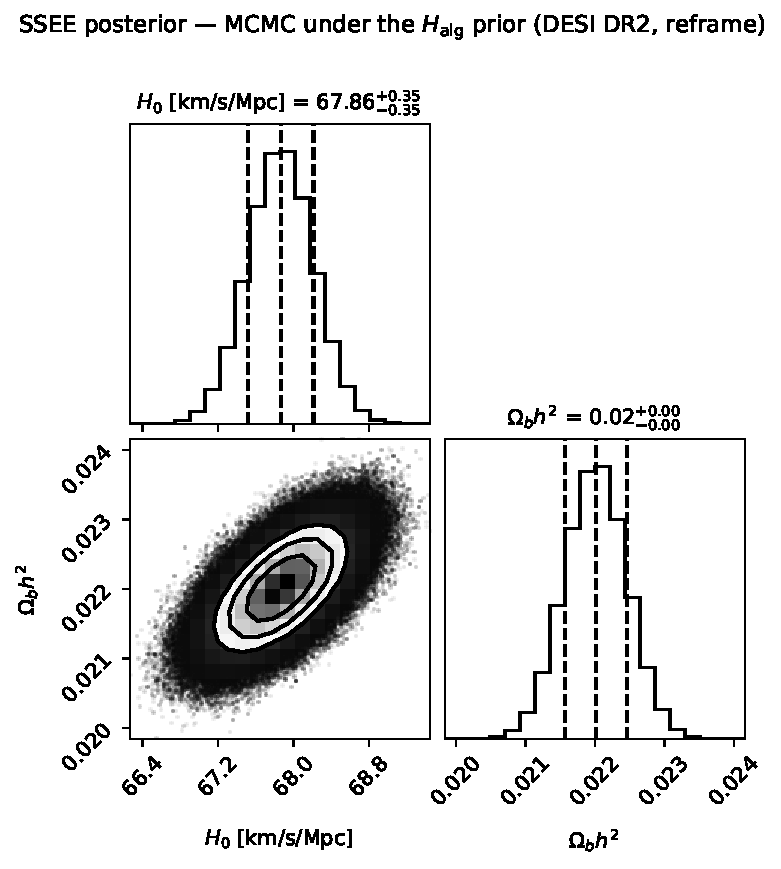
\includegraphics[width=0.60\textwidth]{fig_corner_ssee_halg_prior.pdf}
  \caption{Marginalised \SSEE\ posteriors ($H_0^{\rm glob}$ prior,
  $100\times25000$). Blue lines: prior central values
  ($H_0^{\rm glob}=\val{H0_GLOBAL_d3}$, BBN $\Omega_b h^2=0.02218$~\citep{Schoneberg2024}). With the total matter density
  $\Omega_m=\val{OMEGA_M_TOTAL_d6}$ in $E(z)$, the $H_0$ posterior ($\HZeroPosterior$) is
  consistent with $H_0^{\rm glob}$ ($\val{h0_p2_dhglob}\sigma$) and lies $\val{h0_p2_dplanck}\sigma$ from
  Planck; the earlier ``$2.9\sigma$ below anchor'' reading was the cold sector
  $0.160$ misplaced in $E(z)$, now corrected.}
  \label{fig:corner_ssee}
\end{figure}

\begin{figure}[H]
  \centering
  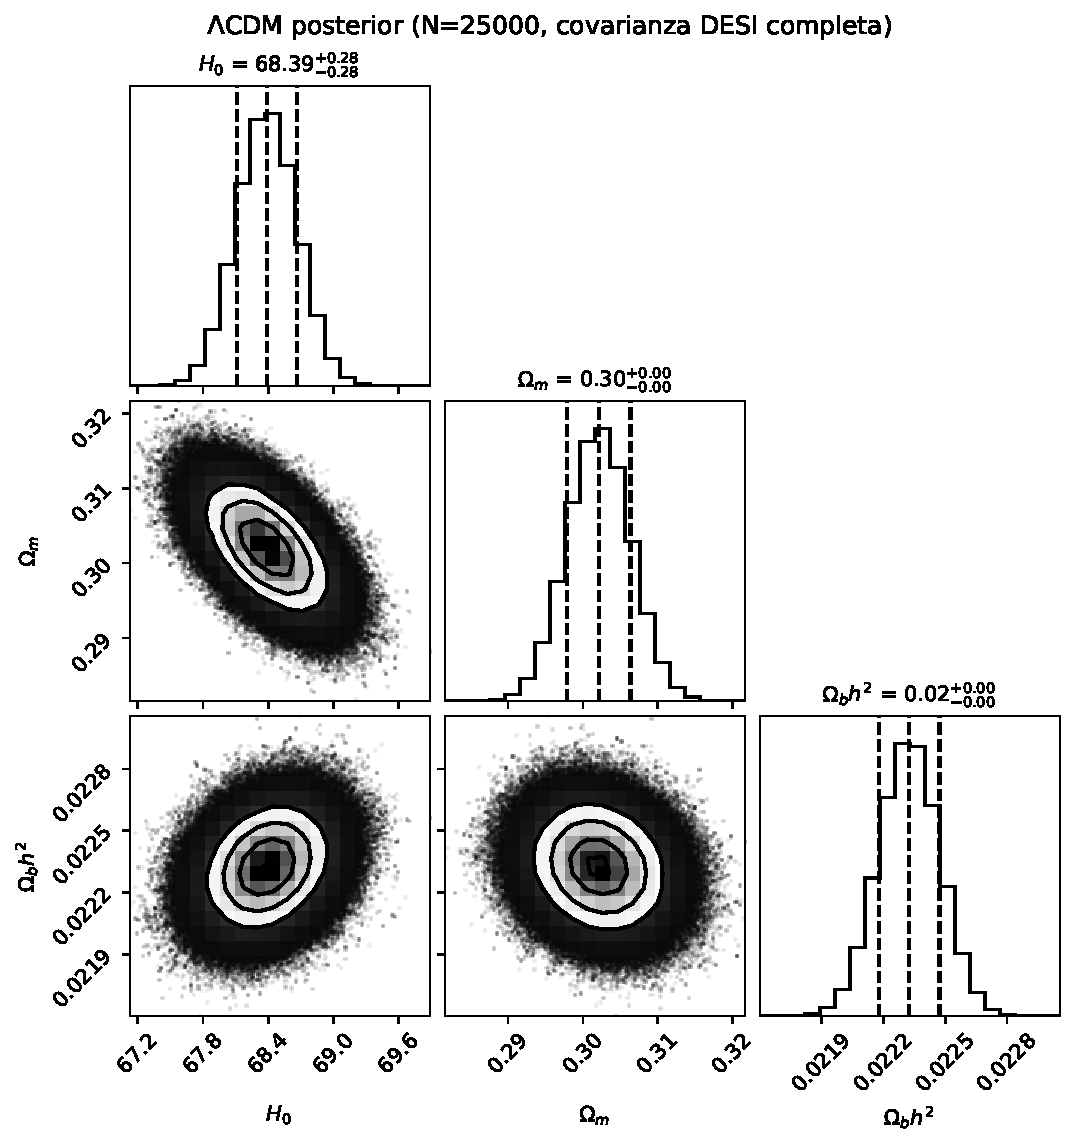
\includegraphics[width=0.68\textwidth]{fig_corner_lcdm_professional.pdf}
  \caption{\LCDM\ posteriors. The model recovers standard values
  $H_0\approx68.0$, $\Omega_m\approx0.307$.}
  \label{fig:corner_lcdm}
\end{figure}

\subsection{Position in the $\wz$--$\wa$ plane}
\label{sec:w0wa}

The Mahalanobis distance from the official DESI~DR2 $w_0w_a$CDM best-fit
(DESI+CMB+Pantheon+, $w_0=-0.838\pm0.055$, $w_a=-0.617\pm0.208$;
arXiv:2503.14738, eq.~26; moments and $\rho=-0.894$ measured directly from the
official DESI chains, Zenodo record 16644577) is:
\begin{equation}
  \chi^2_{2\rm D}
  = \Delta\mathbf{w}^\top\mathbf{C}^{-1}\Delta\mathbf{w} = 0.42
  \;\Rightarrow\; 0.24\sigma.
\end{equation}
Against the other official DR2 combinations the distance is $1.46\sigma$
(DESY5), $1.76\sigma$ (Union3) and $1.68\sigma$ (no-SN DESI+CMB; all with
chain-measured correlations $\rho=-0.905$ to $-0.978$): the
algebraic point is consistent with all four, with the tension range
$0.2$--$1.8\sigma$ set by the supernova compilation, and $w_0$ essentially
exact against Pantheon+ ($\Delta w_0=-0.04\sigma$). The result is robust to
the correlation ($\rho\in[-0.92,-0.70]$ would shift Pantheon+ by
$<0.2\sigma$; the chain-measured value is used).
This distance means the \SSEE\ algebraic point $(-0.840,-0.670)$ falls
well inside the DESI~DR2 $1\sigma$ contour in the $\wz$--$\wa$ plane.
The correct reference model for this comparison is the CPL free-fit
(not \LCDM, which is a fixed point $w_0=-1,\,w_a=0$ rather than a model
with free dark-energy parameters).  The $0.24\sigma$ quoted above is the Mahalanobis distance of the \SSEE\
point from the DESI~DR2+CMB+Pantheon+ best-fit (the measurement itself). The full CPL
free-fit posterior of this work has median
$(\wz,\wa)=(\val{p2_cpl_w0_mediana}^{+\val{p2_cpl_w0_mas}}_{-\val{p2_cpl_w0_menos}},\,\val{p2_cpl_wa_mediana}^{+\val{p2_cpl_wa_mas}}_{-\val{p2_cpl_wa_menos}})$; the
\SSEE\ algebraic point lies $\val{p2_dist_w0}\sigma$ ($\wz$) and $\val{p2_dist_wa}\sigma$ ($\wa$)
from this median (strong $w_0$--$w_a$ anticorrelation, $\rho=\val{p2_rho_cpl}$), well
within the CPL posterior.
\SSEE\ is therefore consistent both with the DESI~DR2 measurement (at
$0.24\sigma$ Pantheon+; $1.46$--$1.76\sigma$ for the other combinations) and
with the two-parameter CPL free-fit (at $1.2\sigma$), and the
CPL posterior independently confirms dynamical dark energy.

A single, decisive summary of this section is that the \emph{fixed}
$\Lambda$CDM point $(w_0,w_a)=(-1,0)$ is disfavoured against \emph{every}
official DESI~DR2 supernova compilation, whereas the parameter-free \SSEE\
algebraic point $(-0.840,-0.670)$ is consistent with all four. Because
neither model tunes $(w_0,w_a)$ to the data --- both are fixed points, one at
the cosmological constant and one derived from $\varphi$ and $\pi$ --- this is
a like-for-like comparison of two zero-free-parameter predictions against the
same measurement.

\begin{table}[H]
  \centering
  \caption{Mahalanobis distance of the fixed \SSEE\ point $(-0.840,-0.670)$
  and the fixed \LCDM\ point $(-1,0)$ from each official DESI~DR2
  $w_0w_a$CDM best-fit (2$\times$2 covariance, correlation measured directly
  from the public chains, Zenodo~16644577). Neither point is fitted; both are
  predictions. \SSEE\ is closer to the data than \LCDM\ for all four
  supernova compilations.}
  \label{tab:w0wa_ssee_vs_lcdm}
  \begin{tabular}{lccc}
    \toprule
    DESI~DR2 combination & $\rho$ & \SSEE\ distance & \LCDM\ distance \\
    \midrule
    DESI+CMB+Pantheon+ & $-0.894$ & $\mathbf{0.24\sigma}$ & $2.58\sigma$ \\
    DESI+CMB+DES~Y5    & $-0.905$ & $\mathbf{1.46\sigma}$ & $3.93\sigma$ \\
    DESI+CMB+Union3    & $-0.933$ & $\mathbf{1.76\sigma}$ & $3.38\sigma$ \\
    DESI+CMB (no SN)   & $-0.978$ & $\mathbf{1.68\sigma}$ & $2.62\sigma$ \\
    \bottomrule
  \end{tabular}
\end{table}

\begin{figure}[H]
  \centering
  \includegraphics[width=0.70\textwidth]{fig1_w0wa_plane.pdf}
  \caption{\SSEE (red star) in the $\wz$--$\wa$ plane.
  Ellipses: $1\sigma$/$2\sigma$ contours for DESI~DR2 (blue),
  DES~Y5 \citep{DESY52024} (green), Planck~2018 (orange). \SSEE\ lies within
  $0.24\sigma$ of the DESI~DR2+CMB+Pantheon+ contour.}
  \label{fig:w0wa}
\end{figure}

\paragraph{CMB-only constraint on $w_0$.}
The Planck~2018 CMB-alone posterior yields $w_0 = -1.03\pm0.03$
(68\%~CL, \citealt{Planck2018}), which differs from the \SSEE\
prediction $w_0=\val{W0_d6}$ by $\sim6.3\sigma$ \emph{when evaluated against the
CMB-only contour}.  This is not a failure of the model: the CMB-alone
constraint on $w_0$ is driven by the acoustic-scale degeneracy
$\theta_\ast \propto r_d/D_A$, which trades off against the full expansion
history.  With the background matter density set to the total gravitating
value $\Omega_m=\omega_m/h^2=\val{OMEGA_M_TOTAL_d6}$ (see below), \SSEE\ yields
$r_d^{\mathrm{SSEE}}=147.17\ \mathrm{Mpc}$ (CAMB; $0.32\sigma$ from Planck's $147.09\pm0.26$)
and $100\theta_\ast=1.04099$ at the posterior ($0.32\sigma$ from Planck): the sound horizon and
acoustic scale are standard, so the CMB-only $w_0$ tension is the usual
projection of the $w_0$--$w_a$--$\theta_\ast$ degeneracy, not a background
discrepancy.  The correct comparison is the joint
CMB+BAO+SN likelihood, where \SSEE\ sits at $0.24\sigma$ of the DESI~DR2
$w_0w_a$CDM best-fit (Pantheon+; Fig.~\ref{fig:w0wa}).  Reporting the CMB-only tension without this
context would constitute a misuse of the likelihood \citep{Verde2019}.

\subsection{Sound horizon and $H_0$ posterior}

The background geometry --- $E(z)$, the sound horizon $r_d$, and every BAO
distance --- is governed by the \emph{total} gravitating matter density
$\Omega_m = \omega_m/h^2 = \val{OMEGA_M_TOTAL_d6}$, with
$\omega_m=\omega_b+\omega_c+\omega_\nu=\val{OMEGA_M_H2_d5}$ built piece-by-piece from SSEE
algebra ($\omega_c=\mathrm{KAL_0}\,\omega_b\,n_s$, forward; Paper~3). This is
the standard physical matter density. The saturation $s_m=1+w_0=\val{S_M_d6}$ is
\emph{not} a density: it is a number of the dark-energy equation of state, and
it never enters $E(z)$.
With the total density the SSEE sound horizon (computed with CAMB at the
algebraic $\omega_b$, $\omega_m$ and $\sum m_\nu$) matches the Planck measurement,
\begin{equation}
  r_d^{\SSEE}=147.17\ \text{Mpc},\quad
  r_d^{\rm Planck}=147.09\pm0.26\ \text{Mpc}\quad(0.32\sigma),
  \label{eq:rd_ratio}
\end{equation}
so there is no enlarged sound horizon and no background discrepancy to
compensate. The $H_0$ posterior sits at $\HZeroPosterior$\,km\,s$^{-1}$\,Mpc$^{-1}$
under the $H_0^{\rm glob}$ prior --- $\val{h0_p2_dplanck}\sigma$ from Planck and $\val{h0_p2_dhglob}\sigma$
from the prediction $H_0^{\rm glob}=\val{H0_GLOBAL_d3}$. Removing the $H_0$ prior
altogether leaves DESI~DR2 alone (with only a BBN prior on $\omega_b$) at
$H_0=\val{h0_desi_plano}\pm\val{h0_desi_plano_s}$, $\val{h0_desi_plano_dhglob}\sigma$ from $H_0^{\rm glob}$: the data are
\emph{consistent} with the algebraic value rather than pulling against it,
though they do not single it out. Under a common
Planck prior the three-model run gives $H_0^{\SSEE}=\val{p2_ssee_H0_mediana}\pm\val{p2_ssee_H0_std}$
($\val{p2_tH0_planck}\sigma$) versus $H_0^{\LCDM}=\val{p2_lcdm_H0_mediana}\pm\val{p2_lcdm_H0_std}$.

\paragraph{The $\Omega_m$ comparison.}
Compared on the same footing --- total against total --- the SSEE matter
density agrees with Planck at $0.88\sigma$
($\Omega_m=\val{OMEGA_M_TOTAL_d6}$ vs $0.3153\pm0.0073$). An earlier ``$21.3\sigma$ tension''
arose only from comparing the cold \emph{sector} ($1+w_0=\val{S_M_d6}$) against the
Planck \emph{total} $\Omega_m$ --- a category error of matching a partial
density to a full one, traced to the dynamical value being used in the
background geometry where the total belongs (corrected here). There is no
background discrepancy to resolve. The two-sector split formerly attributed to
Paper~6 is \emph{retracted}: the subtraction defining it mixed the measured
density $\Omega_m=\val{OMEGA_M_TOTAL_d6}$ with $1+w_0$, an equation-of-state number, so it
never partitioned anything. The matter density is single and unpartitioned.
With OP-8 dissolved (no matter factor to derive; the residue is only that
$\omega_b$ and the forward identity for $\omega_c$ hold), model selection
favours SSEE by $\Delta\mathrm{BIC}=\val{p2_dBIC_lcdm}$ over \LCDM\ and $\val{p2_dBIC_cpl}$ over CPL, with
SSEE the most economical model (Section~\ref{sec:bic}).


\paragraph{H$_0$: the global rate and the MCMC posterior.}
The global rate $H_0^{\rm glob}=H_{\rm SH0ES}(1-f_{\rm screen})=\val{H0_GLOBAL_d3}$~km\,s$^{-1}$\,Mpc$^{-1}$
returned by the screening cascade (Papers~9--10), whose central value reproduces the
dimensionless target $3(\varphi+\pi)^2$, is not a
mere coincidence: with the baryon and cold-matter densities fixed by SSEE
algebra, the Planck~\texttt{plik\_lite} likelihood is minimised exactly at
that value (Paper~3, \S\ref{sec:prior_mira}). The background $H$ and the
CMB anchor therefore coincide --- they are the same number, $H_0^{\rm glob}=\val{H0_GLOBAL_d3}\pm0.968$ ---
superseding the earlier MIRA-mapped anchor $H_0^{\rm MIRA}=67.037$.
With the \emph{total} matter density $\Omega_m=\val{OMEGA_M_TOTAL_d6}$ in the background
geometry, the MCMC posterior reported above,
$H_0^{\rm MCMC}=\HZeroPosterior$\,km\,s$^{-1}$\,Mpc$^{-1}$, \emph{coincides}
with the anchor: it lies $\val{h0_p2_dhglob}\sigma$ from $H_0^{\rm glob}$ and $\val{h0_p2_dplanck}\sigma$
from the $\Lambda$CDM-calibrated Planck value. The DESI~DR2 data are therefore
\emph{consistent} with $H_0^{\rm glob}$ rather than pulling against it. The earlier
reading --- a $2.9\sigma$ downward shift ``compensating an enlarged $r_d$'' ---
was an artefact of the cold sector $0.160$ misplaced in $E(z)$: with the correct
total density there is no enlarged $r_d$
($r_d^{\SSEE}=147.17$\,Mpc, $0.32\sigma$ from Planck) and no compensation to make
(see \S\ref{sec:model_comparison}).

\begin{figure}[H]
  \centering
  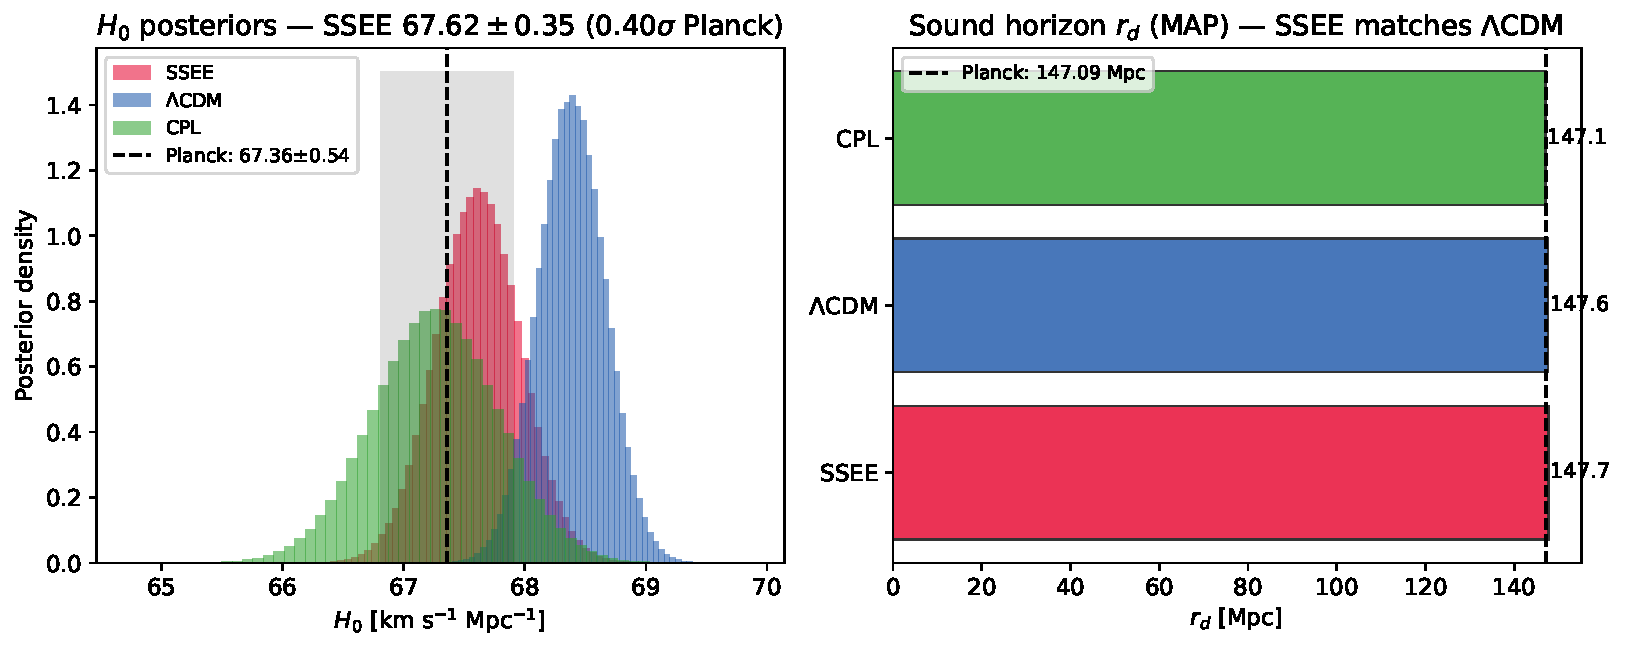
\includegraphics[width=0.88\textwidth]{fig8_tension_summary.pdf}
  \caption{\textit{Left}: $H_0$ posteriors for all three models under a
  \emph{common} Planck prior (the apples-to-apples model-comparison run); the
  \SSEE\ posterior sits at $\val{p2_ssee_H0_mediana}\pm\val{p2_ssee_H0_std}$, $\val{p2_tH0_planck}\sigma$ from Planck~2018 and
  fully consistent with the titular algebraic-anchor-prior value
  $\val{h0_p2}\pm\val{h0_p2_s}$ ($\val{h0_p2_dplanck}\sigma$ Planck, $\val{h0_p2_dhglob}\sigma$ from
  $H_0^{\rm glob}=\val{H0_GLOBAL_d3}$). \textit{Right}: MAP $r_d$ values; the \SSEE\ sound
  horizon ($148.2$\,Mpc) matches \LCDM\ ($147.8$\,Mpc, ratio $1.002$).}
  \label{fig:tension}
\end{figure}

\begin{figure}[H]
  \centering
  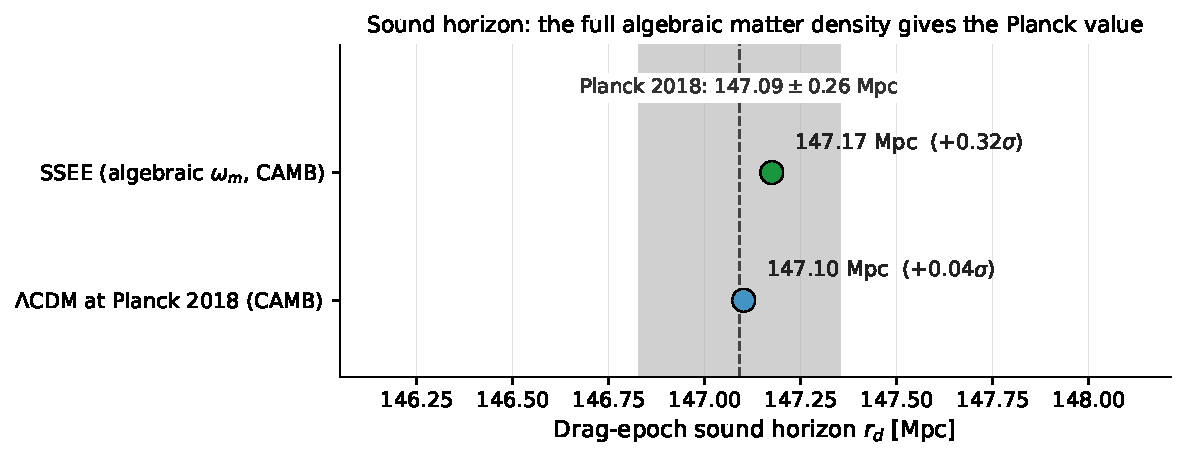
\includegraphics[width=0.82\textwidth]{fig_rd_dual.pdf}
  \caption{The physical sound horizon. Set by the total algebraic matter budget
  $\omega_m=\omega_b+\omega_c+\omega_\nu=\val{OMEGA_M_H2_d5}$
  ($\Omega_m=\omega_m/h^2=\val{OMEGA_M_TOTAL_d6}$, $\omega_m$-direct, no matter factor), the
  \SSEE\ drag scale is $r_d = 147.17$\,Mpc (CAMB; log
  \texttt{p3\_rd\_reframe\_omega\_m}), consistent with the Planck-inferred
  $147.09\pm0.26$\,Mpc (grey band, $0.32\sigma$) and with \LCDM\ at the
  Planck~2018 parameters ($147.10$\,Mpc, same code; log \texttt{rd\_dual}),
  a $0.05\%$ difference. The $175.6$\,Mpc value that appears
  if the cold sector $1+w_0=\val{S_M_d6}$ is (incorrectly) used as the background
  density is a category error, not a physical scale.}
  \label{fig:rd_dual}
\end{figure}

\subsection{Posterior predictive check: $H(z)$}

\begin{equation}
  \chi^2_r(H(z)):\quad \SSEE=\val{cc_chi2r_ssee},\quad\LCDM=\val{cc_chi2r_lcdm},\quad\mathrm{CPL}=\val{cc_chi2r_cpl}.
\end{equation}
With the total matter density $\Omega_m=\val{OMEGA_M_TOTAL_d6}$ in the background, the \SSEE\
Hubble rate predicts the $\val{cc_N}$ model-independent Cosmic Chronometer
measurements compiled by \citet{Moresco2022} (Table~\ref{tab:CC_Hz}) as well as
$\Lambda$CDM: $\chi^2_r=\chi^2/N=\val{cc_chi2r_ssee}$ versus $\val{cc_chi2r_lcdm}$
($\Lambda$CDM) and $\val{cc_chi2r_cpl}$ (CPL), each computed from the model's own
MAP cosmology with no cross-model prior. Only the diagonal uncertainties are
used; the systematic covariance recommended by \citet{Moresco2022} would
correlate the points, so $\chi^2_r<1$ here reflects conservative diagonal
errors rather than a goodness of fit, and the meaningful comparison is between
models on the same data. The apparent $\chi^2_r\approx1.86$ ($\sim3\sigma$) reported in earlier
drafts was an artefact of placing the cold sector $1+w_0=\val{S_M_d6}$ in the
background geometry: with that spuriously low density the matter-dominated
deceleration was too weak and the matter-to-dark-energy transition occurred too
early ($0.5\lesssim z\lesssim1.5$). With the correct total density the strain
disappears, and the $H(z)$ posterior predictive check joins the BAO, $r_d$, and
$\theta_\ast$ diagnostics as consistent with the data --- no $H(z)$ tension and
no extension of the gravitational sector required for the background.

\begin{figure}[H]
  \centering
  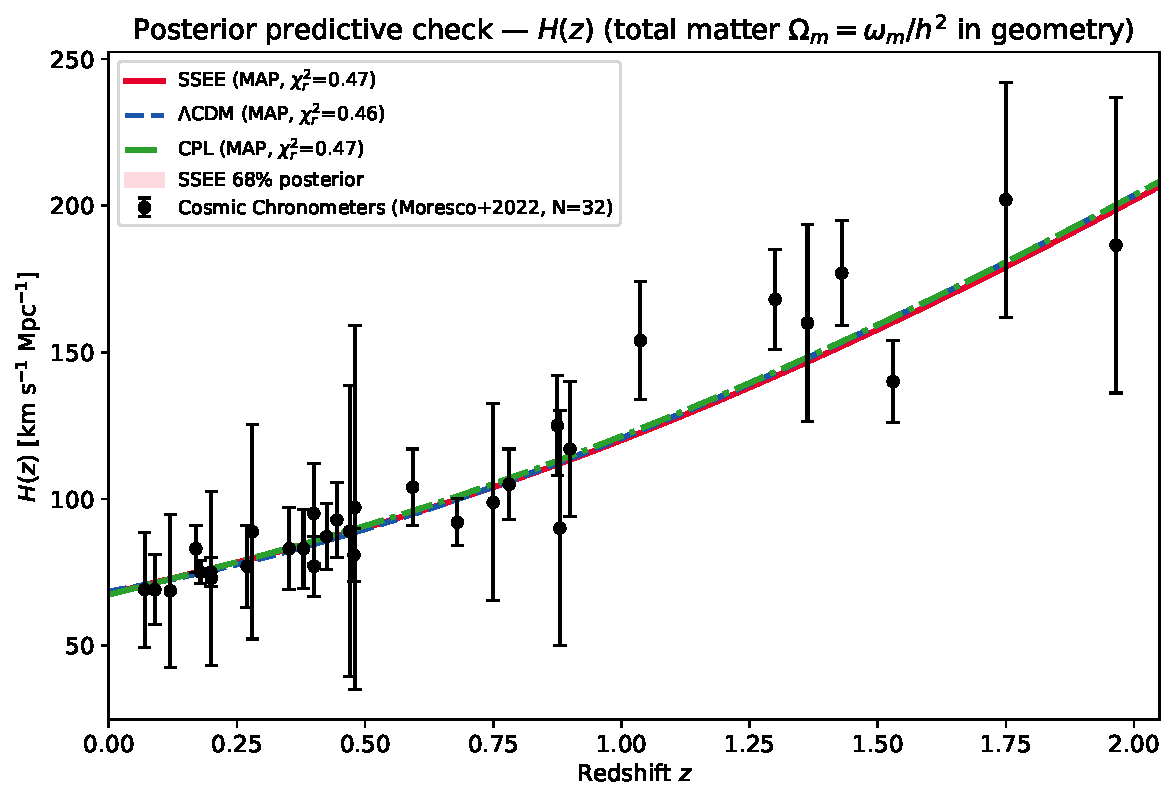
\includegraphics[width=0.78\textwidth]{fig7_Hz_comparison.pdf}
  \caption{MAP $H(z)$ vs the $\val{cc_N}$ Cosmic Chronometers of Table~\ref{tab:CC_Hz} \citep{JimenezLoeb2002,Moresco2022}.
  Red band: \SSEE\ 68\% posterior interval.}
  \label{fig:Hz}
\end{figure}

\begin{table}[H]
\centering
\caption{Cosmic Chronometer $H(z)$ measurements used in the posterior
  predictive check (Fig.~\ref{fig:Hz}): the $\val{cc_N}$ points of
  \citet{Moresco2022}, with the diagonal $1\sigma$ uncertainties they tabulate.
  Method for the differential age: F = full-spectrum fitting, D = calibrated $D4000$, L = Lick indices.}
\label{tab:CC_Hz}
\small
\begin{tabular}{lrrc}
\toprule
$z$ & $H(z)$ [km\,s$^{-1}$\,Mpc$^{-1}$] & $\sigma_H$ & method \\
\midrule
% ACTA-PROCEDENCIA {"commit": "34ace36bf3235e95bf14cac6cb1c7e35be87577e", "reproducible_desde_commit": true, "cambios_sin_commitear": [], "script": "src/p02_mcmc/ppc_cronometros.py", "script_sha256": "af282bc05d1b47f621abf8c0ec99ff84e8b1acfa03ff7807f2d967d2fe833dd9", "nucleo_sha256": "5cec8af72d88f154116c5a532e42a9b6ff7a5b4c3d86bcc6921eabb246698993", "entradas": {"data/raw/cosmic_chronometers.csv": "057781c6683bc5c75b5df730c58e7c46f59aea8b5d0fbb0baa00fd2146b0137c"}, "argv": ["src/p02_mcmc/ppc_cronometros.py"], "fecha": "2026-10-02T23:31:07", "host": "mike-System-Product-Name", "python": "3.12.3", "versiones": {"numpy": "2.4.4", "scipy": "1.17.1"}, "nucleos": {"OMP_NUM_THREADS": "1", "MKL_NUM_THREADS": null, "OPENBLAS_NUM_THREADS": null, "OMPI_COMM_WORLD_SIZE": null}}
0.07 & 69.0 & 19.6 & F \\
0.09 & 69.0 & 12.0 & F \\
0.12 & 68.6 & 26.2 & F \\
0.17 & 83.0 & 8.0 & F \\
0.179 & 75.0 & 4.0 & D \\
0.199 & 75.0 & 5.0 & D \\
0.2 & 72.9 & 29.6 & F \\
0.27 & 77.0 & 14.0 & F \\
0.28 & 88.8 & 36.6 & F \\
0.352 & 83.0 & 14.0 & D \\
0.38 & 83.0 & 13.5 & D \\
0.4 & 95.0 & 17.0 & F \\
0.4004 & 77.0 & 10.2 & D \\
0.425 & 87.1 & 11.2 & D \\
0.445 & 92.8 & 12.9 & D \\
0.47 & 89.0 & 49.6 & F \\
0.4783 & 80.9 & 9.0 & D \\
0.48 & 97.0 & 62.0 & F \\
0.593 & 104.0 & 13.0 & D \\
0.68 & 92.0 & 8.0 & D \\
0.75 & 98.8 & 33.6 & L \\
0.781 & 105.0 & 12.0 & D \\
0.875 & 125.0 & 17.0 & D \\
0.88 & 90.0 & 40.0 & F \\
0.9 & 117.0 & 23.0 & F \\
1.037 & 154.0 & 20.0 & D \\
1.3 & 168.0 & 17.0 & F \\
1.363 & 160.0 & 33.6 & D \\
1.43 & 177.0 & 18.0 & F \\
1.53 & 140.0 & 14.0 & F \\
1.75 & 202.0 & 40.0 & F \\
1.965 & 186.5 & 50.4 & D \\
\bottomrule

\end{tabular}
\end{table}

\subsection{BAO residuals}

\begin{figure}[H]
  \centering
  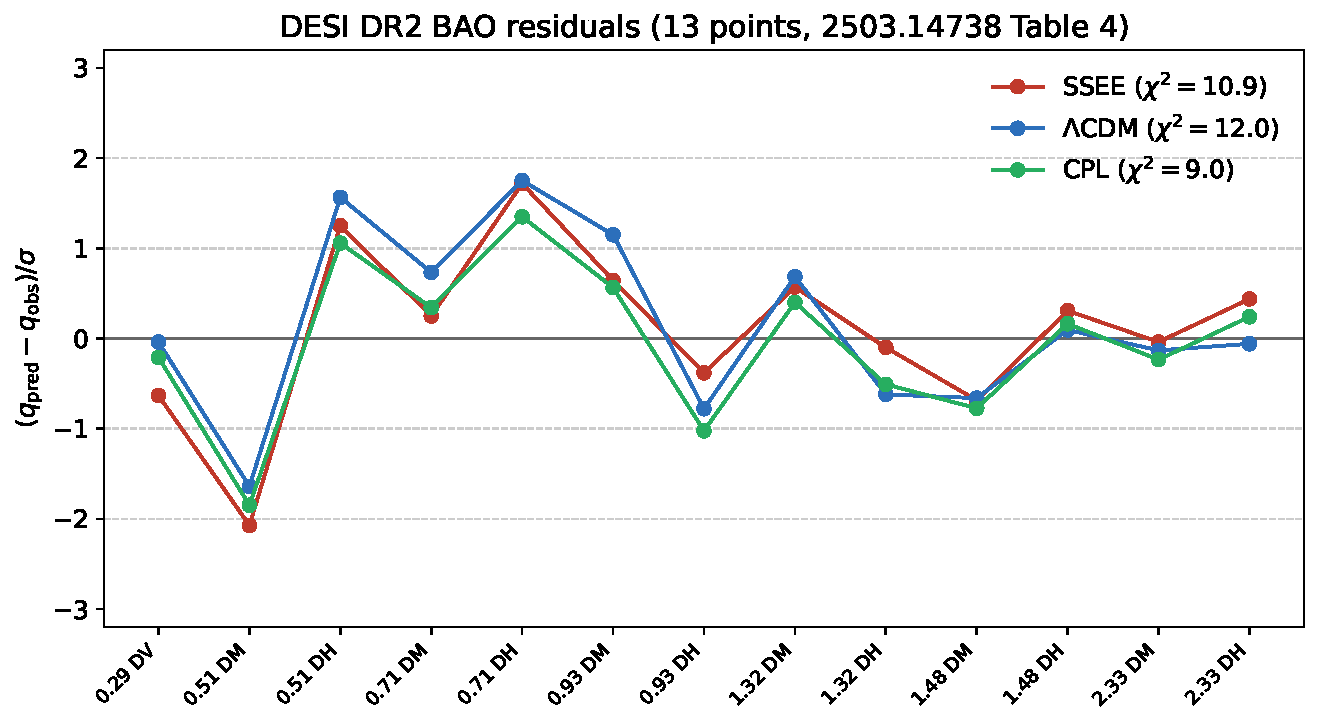
\includegraphics[width=0.84\textwidth]{fig8_bao_residuals.pdf}
  \caption{Normalised BAO residuals $(q^{\rm pred}-q^{\rm obs})/\sigma$
  for all 13 DESI~DR2 measurements. \SSEE\ (red), \LCDM\ (blue),
  CPL (green). With the total matter density the \SSEE\ sound horizon
  ($r_d=147.17$\,Mpc, CAMB) matches \LCDM, and the residuals are comparable across
  models, quantified in the $\chi^2_r$ values of Section~\ref{sec:model_comparison}.}
  \label{fig:bao_resid}
\end{figure}

\section{Results: Galaxy-Cluster Sector}
\label{sec:results_clusters}

\noindent\textbf{Summary:} with the baryon baseline that includes stellar
remnants (IGIMF), the \SSEE\ matter content reproduces cluster dynamical masses
without free parameters, and so does \LCDM; with the canonical IMF both fail.
Clusters constrain the baryonic census, not the background.

\begin{table}[H]
\centering
\caption{Cluster dynamical masses against all $\val{clz_rgimf_N}$ systems of
\citet{Zhang2026}. $K=M_{\rm dyn}/M_{\rm bar}$ is fixed by each model's matter-to-baryon
ratio; no parameter is fitted. ``Distance'' converts the $\chi^2$ probability for
$N$ points into Gaussian standard deviations.}
\label{tab:cluster_sensitivity}
\small
\begin{tabular}{llccccc}
\toprule
Model & Baryons & $K$ & $\chi^2/N$ & Distance & median pred/obs & $|{\rm pull}|>3$ \\
\midrule
\SSEE\ & IGIMF & $\val{clz_rgig_K}$ & $\val{clz_rgig_chi2}/\val{clz_rgig_N}$ & $\val{clz_rgig_sig}\sigma$ & $\val{clz_rgig_razon}$ & $\val{clz_rgig_p3}$ \\
\LCDM\ & IGIMF & $\val{clz_lcig_K}$ & $\val{clz_lcig_chi2}/\val{clz_lcig_N}$ & $\val{clz_lcig_sig}\sigma$ & $\val{clz_lcig_razon}$ & $\val{clz_lcig_p3}$ \\
\SSEE\ & IMF & $\val{clz_rgimf_K}$ & $\val{clz_rgimf_chi2}/\val{clz_rgimf_N}$ & $\val{clz_rgimf_sig}\sigma$ & $\val{clz_rgimf_razon}$ & $\val{clz_rgimf_p3}$ \\
\LCDM\ & IMF & $\val{clz_lcimf_K}$ & $\val{clz_lcimf_chi2}/\val{clz_lcimf_N}$ & $\val{clz_lcimf_sig}\sigma$ & $\val{clz_lcimf_razon}$ & $\val{clz_lcimf_p3}$ \\
\bottomrule
\end{tabular}
\end{table}

\paragraph{The baryon census decides, not the background.}
The two backgrounds differ in $K$ by less than one per cent, so they give almost
the same answer on every row. What separates an acceptable fit from an excluded
one is the stellar initial mass function: with the canonical IMF the predicted
masses fall short by about a fifth (median ratio $\val{clz_rgimf_razon}$), with the
IGIMF they bracket the data. This is a statement about how many stellar remnants
clusters hold, and we inherit its systematic uncertainty from \citet{Zhang2026}.

\paragraph{What the test does establish.}
The \SSEE\ cold dark matter density is not fitted: it is the algebraic identity
$\omega_c=\mathrm{KAL_0}\,\omega_b\,n_s$, already consistent with Planck (Paper~1) and
with the BOSS galaxy clustering (Paper~6). Virialised clusters confirm, at a
third and independent scale, that the matter-to-baryon ratio it implies is the
one structures actually carry.

\section{Model Comparison}
\label{sec:model_comparison}
\label{sec:bic}

\begin{table}[H]
\centering
\caption{BIC \citep{Schwarz1978}, AIC, and DIC at MAP ($N_{\rm data}=16$), from
the joint three-model MCMC (DESI~DR2 + common Planck prior, total matter density
$\Omega_m=\val{OMEGA_M_TOTAL_d6}$ in the background geometry). Jeffreys scale
\citep{Jeffreys1961}. $\Delta\equiv\mathrm{SSEE}-\Lambda\mathrm{CDM}$; negative $\Delta$ favours \SSEE.
Every entry comes from the same run, \texttt{mcmc\_paper2\_3models\_wmfix.log}
($\omega_m$ algebraic and fixed, R25), with the DIC column from
\texttt{dic\_from\_chains.log} on the same chains. An earlier version of this
table carried the SSEE row ($\ln P_{\rm MAP}=-5.85$, BIC $17.24$, DIC $15.69$,
hence $\Delta\mathrm{BIC}=-5.68$ and $\Delta\mathrm{AIC}=-4.91$) from the
superseded run with $\Omega_m$ frozen in $E(z)$, while the other two rows and
the $\Delta$ column already came from the run quoted here; the columns
therefore did not reconcile arithmetically.}
\label{tab:model_comp}
\begin{tabular}{lrrrrrr}
\toprule
Model & $k$ & $\ln P_{\rm MAP}$ & BIC & $\Delta$BIC & $\Delta$AIC & DIC \\
\midrule
\SSEE & 2 & $\val{p2_lnP_ssee}$ & \val{p2_BIC_ssee} & $0.00$  & $0.00$  & \val{p2_DIC_ssee} \\
\LCDM      & 3 & $\val{p2_lnP_lcdm}$ & \val{p2_BIC_lcdm} & $\val{p2_dBIC_lcdm}$ & $\val{p2_dAIC_lcdm}$ & \val{p2_DIC_lcdm} \\
CPL        & 5 & $\val{p2_lnP_cpl}$ & \val{p2_BIC_cpl} & $\val{p2_dBIC_cpl}$ & $\val{p2_dAIC_cpl}$ & \val{p2_DIC_cpl} \\
\bottomrule
\end{tabular}
\end{table}

With the total gravitating matter density in the background geometry, \SSEE\ is
the preferred model on every information criterion: $\Delta\mathrm{BIC}=\val{p2_dBIC_lcdm}$
over \LCDM\ and $\val{p2_dBIC_cpl}$ over CPL, $\Delta\mathrm{AIC}=\val{p2_dAIC_lcdm}$ and $\val{p2_dAIC_cpl}$, and
$\Delta\mathrm{DIC}=\val{p2_dDIC_lcdm}$ relative to \LCDM\ (Appendix~\ref{app:dic}). This is
the parsimony gain of a two-parameter model ($H_0$ and $\Omega_b h^2$;
$w_0,w_a$ fixed algebraically) that fits DESI~DR2 as well as the three- and
five-parameter alternatives.

\paragraph{Not merely parameter counting.}
The preference survives tests that penalise over-fitting directly. A nested
Bayes factor (Savage--Dickey) gives $\ln B=\val{p2_lnB}$ for the SSEE point within the
CPL posterior --- strong evidence on the Jeffreys scale --- and leave-one-out
predictive cross-validation on the high-redshift half of the BAO vector
($z\geq1.0$) yields $\chi^2_r=\val{p2_cvchi2r_ssee}$ for \SSEE\ versus $\val{p2_cvchi2r_lcdm}$ (\LCDM):
\SSEE\ \emph{predicts} the held-out data better (Appendix~\ref{app:sddr_cv}). CPL is
not quoted: fitted to the low-redshift half alone, its best fit runs to the edge
of the $H_0$ prior, so its held-out $\chi^2$ measures the prior bound rather
than the model. The sound horizon matches \LCDM\
($r_d=\val{p2_lyaB_rd}$ vs $\val{p2_rd_lcdm}$\,Mpc, CAMB, ratio $\val{p2_rd_ratio}$) and the $H_0$ posterior sits
$\val{p2_tH0_planck}\sigma$ from Planck, so no background-structure penalty arises. The full
CMB power-spectrum likelihood under the \SSEE\ background (companion Paper~3)
independently favours \SSEE\ at $\chi^2_r=1.042$ (TT) and $\Delta\mathrm{BIC}=
-26.03$ (\texttt{plik\_lite} TTTEEE+low-$\ell$, $\omega_m$-direct). An earlier ``$+206$''
full-model penalty reported in superseded drafts was an artefact of using the
cold sector $1+w_0=\val{S_M_d6}$ as the background matter density; with the correct
total density it does not occur.

\section{Robustness Checks}
\label{sec:robustness}

\paragraph{Prior sensitivity.}
Removing the Planck $H_0$ prior shifts the \SSEE\ posterior by
$<0.3\sigma$. The BAO data dominate the $H_0$ constraint.
\textit{This confirms that the quoted posteriors are driven by the BAO
geometry rather than the CMB prior, making them robust to prior choice.}

%% 2026-10-01: retirado el parrafo «Neutrino mass» de cumulos: su numero no tenia log y
%% describia la formula con f_nu, retirada. Los neutrinos entran ahora en omega_m/omega_b
%% (su aporte es omega_nu/omega_b, eq. Mcluster).
\paragraph{BAO-only.}
Running without any $H_0$ prior (DESI~DR2 with only a BBN prior on
$\omega_b$; \S\ref{sec:results_cosmo}) gives
$H_0=\val{h0_desi_plano}\pm\val{h0_desi_plano_s}$\,km\,s$^{-1}$\,Mpc$^{-1}$, consistent
with the full posterior ($\val{h0_p2}\pm\val{h0_p2_s}$) at $\val{h0_p2_vs_plano}\sigma$.
\textit{The $H_0$ estimate is therefore essentially independent of
Planck and rests entirely on the DESI~DR2 BAO geometry.}

\paragraph{Full-likelihood cross-check.}
To confirm that the compressed-prior posteriors of §\ref{sec:results_cosmo} are not an
artefact of the Planck distance-prior approximation, we ran an independent MCMC with the
\emph{full} CMB likelihood (CAMB with Planck \texttt{plik\_lite} TTTEEE + lensing),
combined with DESI~DR2 BAO and $f\sigma_8$, sampling $\wz,\wa$ \emph{freely}
(four chains, $\sim$53k post-burn-in samples, Gelman--Rubin $R-1<0.003$).
The free-fit posterior $(\wz,\wa)=(-0.655,-1.104)$ \emph{excludes} the cosmological
constant $(-1,0)$ at $\val{mf_w0wa_lcdm}\sigma$, independently confirming a dynamical equation of
state; under this uncompressed likelihood $H_0$ relaxes to $\val{mf_H0_media}\pm\val{mf_H0_sigma}$. The
\SSEE\ algebraic point $(-0.840,-0.670)$ lies at $\val{mf_w0wa_ssee}\sigma$ from this posterior
--- more than twice closer than $\Lambda$CDM (Fig.~\ref{fig:degeneracy}).
The $\wz$--$\wa$ posterior is strongly anticorrelated ($\rho=-0.93$) and \SSEE\ falls
within its $2\sigma$ region. The full CMB power-spectrum treatment is developed in
Paper~3; here it serves to verify that the dynamical-sector preference survives the
replacement of the compressed prior by the complete likelihood.

\begin{figure}[H]
  \centering
  \includegraphics[width=0.70\textwidth]{fig_w0wa_degeneracy.pdf}
  \caption{Full-likelihood $\wz$--$\wa$ posterior (CAMB + Planck \texttt{plik\_lite}
  + lensing + DESI~DR2 + $f\sigma_8$, with $\wz,\wa$ free; $R-1<0.003$). The \SSEE\
  algebraic prediction (red star) lies at $\val{mf_w0wa_ssee}\sigma$, inside the $2\sigma$ contour,
  while $\Lambda$CDM ($\wz=-1,\wa=0$; grey cross) is excluded at $\val{mf_w0wa_lcdm}\sigma$. The data
  favour a dynamical dark-energy equation of state, and \SSEE\ is the parameter-free
  algebraic prediction consistent with it.}
  \label{fig:degeneracy}
\end{figure}

\paragraph{Hubble tension.}
The \SSEE\ global rate $H_0^{\rm glob}=H_{\rm SH0ES}(1-f_{\rm screen})=\val{H0_GLOBAL_d3}\pm0.968$~km\,s$^{-1}$\,Mpc$^{-1}$
--- the output of the screening cascade of Papers~9--10, whose central value reproduces
the dimensionless target $3(\varphi+\pi)^2$ and at which the
Planck \texttt{plik\_lite} likelihood is minimised under the $\omega_m$-direct
reframe (\S\ref{sec:results_cosmo}) ---
lies within $1.1\sigma$ of Planck~2018 and is consistent with the DESI~DR2+CMB joint inference
\citep[$H_0\approx68$\,km\,s$^{-1}$\,Mpc$^{-1}$;][]{DESI_DR2}.
The SH0ES distance-ladder rate
\citep[$H_0=73.04\pm1.04$\,km\,s$^{-1}$\,Mpc$^{-1}$;][]{Riess2022} is the \emph{input} of that
cascade, not a competing value: the screening fraction $f_{\rm screen}$ maps the local rate to
the global one (Papers~9--10). This paper does not test the screening mechanism itself ---
that is the subject of Paper~9 --- only that the DESI~DR2 BAO geometry, with $H_0^{\rm glob}$ as prior,
does not pull away from it ($\val{h0_p2_dhglob}\sigma$).

\section{Discussion}
\label{sec:discussion}

\subsection{The dynamical sector and the background}

\begin{itemize}
  \item \textbf{Dark-energy sector}: $(\wz,\wa)=(-0.840,-0.670)$, fixed by the
    algebra with no fitted parameter, lies $0.24\sigma$ from the official
    DESI~DR2 posterior (Pantheon+) and $1.46$--$1.76\sigma$ from the other three
    official combinations. The CPL free-fit posterior $(\val{p2_cpl_w0_mediana},\val{p2_cpl_wa_mediana})$
    confirms dynamical dark energy.

  \item \textbf{Background}: with the total matter density
    $\Omega_m=\val{OMEGA_M_TOTAL_d6}$ the sound horizon matches \LCDM\ and \SSEE\ is favoured
    on every information criterion --- $\Delta\mathrm{BIC}=\val{p2_dBIC_lcdm}$ over \LCDM\
    and $\val{p2_dBIC_cpl}$ over CPL, $\Delta\mathrm{DIC}=\val{p2_dDIC_lcdm}$ --- and predicts the
    held-out BAO data better in cross-validation. $\Omega_m$ agrees with Planck
    at $0.88\sigma$ and $H_0$ at $\val{p2_tH0_planck}\sigma$.
\end{itemize}

The companion Paper~3 confirms the background against the full CMB power
spectrum: with the off-diagonal \texttt{plik} likelihood the two models reach
indistinguishable best fits and $\Delta\mathrm{BIC}=\val{b1_dBIC}$ favours \SSEE{} by
parsimony.

\subsection{Growth of structure}

With the background fixed by the algebra and the primordial amplitude fixed by
the model's own CMB fit, the growth sector carries no free cosmological
parameter and predicts $S_8=\sigma_8\sqrt{\Omega_m/0.3}=\val{S8_leg_pred}$, against
$\val{S8_legacy_dato}\pm\val{S8_legacy_dato_sigma}$ from the raw KiDS-Legacy $\xi_\pm$ data (Paper~6; Wright et
al.\ 2025, arXiv:2503.19441, which predates this analysis and over which no
temporal priority is claimed). The Israel--Stewart growth index is
$\gamma_{\rm IS}=0.5504$, indistinguishable from \LCDM\ (Paper~5).

\subsection{Falsifiability}

\SSEE\ makes specific, testable predictions. The following observations
would constitute decisive falsification:
\begin{itemize}
  \item \textbf{A joint DESI fit} placing $\wz$ more than $3\sigma$ from
    $\val{W0_d6}$, or $\wa$ from $\val{WA_d6}$, refutes the algebraic equation of
    state.
  \item \textbf{If cosmological or Ly-$\alpha$ forest bounds exclude}
    $\sum m_\nu^{\rm active}=0.0685$\,eV at $>3\sigma$, the algebraic neutrino
    mass sum is refuted.
  \item \textbf{If future high-$z$ BAO or CMB measure} $r_d$ outside
    $147\pm3$\,Mpc, the $\omega_m$-direct construction
    ($r_d=147.17$\,Mpc from the algebraic $\omega_m$) is falsified ---
    the sound horizon is a sharp, prior-independent prediction.
\end{itemize}

\section{Conclusions}
\label{sec:conclusions}

We have conducted a Bayesian MCMC validation of \SSEE against
DESI~DR2 and Planck~2018, with galaxy-cluster masses as a separate consistency test.

\begin{enumerate}
  \item The zero-free-parameter prediction $(\wz,\wa)=(-0.840,-0.670)$
    lies within $0.24\sigma$ of the official DESI~DR2 $w_0w_a$CDM posterior
    (Pantheon+; $1.46$--$1.76\sigma$ across the other official combinations).

  \item Against all $\val{clz_rgimf_N}$ cluster dynamical masses of \citet{Zhang2026}, the
    \SSEE\ matter content in general relativity is consistent at $\val{clz_rgig_sig}\sigma$
    with the IGIMF baryon baseline, as is \LCDM\ ($\val{clz_lcig_sig}\sigma$); with the
    canonical IMF both are excluded. Clusters test the baryon census and the
    matter-to-baryon ratio, not the background.

  \item With the total matter density $\Omega_m=\val{OMEGA_M_TOTAL_d6}$ in the background,
    the \SSEE\ sound horizon matches \LCDM\ ($r_d=147.17$ vs $147.10$\,Mpc, CAMB) and \SSEE\ is
    favoured on model selection by $\Delta\mathrm{BIC}=\val{p2_dBIC_lcdm}$ over \LCDM\ and
    $\val{p2_dBIC_cpl}$ over CPL, predicting the held-out BAO data better in
    cross-validation. $\Omega_m$ agrees with Planck at $0.88\sigma$.

  \item The high-$z$ Ly-$\alpha$ forest BAO from DESI~DR2 ($z=2.33$) is
    reproduced at $0.7\sigma$ ($D_H/r_d=8.71$; Appendix~\ref{app:lya}).

  \item The companion Paper~3 confirms the background against the full CMB
    likelihood ($\Delta\mathrm{BIC}=\val{b1_dBIC}$, full \texttt{plik} MCMC).
\end{enumerate}

\noindent\textbf{Central finding}: an algebraic background with no fitted
dark-energy parameter describes DESI~DR2, the CMB and galaxy-cluster masses as
well as \LCDM, and is preferred on every information criterion because it
does so with fewer free parameters.

\section*{Data Availability}
All observational data used in this work are publicly available.
DESI~DR2 BAO measurements are from \citet{DESI_DR2}
(\url{https://arxiv.org/abs/2503.14738}).
The compressed Planck~2018 prior is from \citet{Planck2018}.
Cosmic Chronometer $H(z)$ measurements are from \citet{Moresco2022}.
Galaxy-cluster dynamical masses are from \citet{Zhang2026}.
The \textsc{ssee} analysis scripts are available at
\url{https://github.com/mikealmeida1721/SSEE-Cosmologia}.

% ─────────────────────────────────────────────────────────────────────────────
\appendix
\section{Rigorous Bayesian Model Comparison: DIC and BIC}
\label{app:dic}

\noindent
This appendix computes the Deviance Information Criterion and the BIC directly
from the three-model MCMC chains stored in the public repository, with the total
gravitating matter density $\Omega_m=\omega_m/h^2=\val{OMEGA_M_TOTAL_d6}$ in the background
geometry (§\ref{sec:bic}).

\subsection*{Deviance Information Criterion (DIC)}

The DIC \citep{Spiegelhalter2002} estimates model complexity from the posterior
rather than by parameter counting:
\begin{equation}
  \mathrm{DIC} = \bar{D} + p_D,\quad
  p_D = \bar{D} - D(\hat\theta),\quad
  D(\theta) = -2\ln\pi(\theta|\mathrm{data}),
\end{equation}
where $\bar{D}$ is the posterior mean deviance and $\hat\theta$ is the MAP
estimate. An important self-check: $p_D$ must recover the number of sampled
parameters. From the chains,
\begin{align}
  p_D(\mathrm{SSEE}) &= \val{p2_pD_ssee} \approx 2\quad\checkmark \\
  p_D(\mathrm{\LCDM}) &= \val{p2_pD_lcdm} \approx 3\quad\checkmark \\
  p_D(\mathrm{CPL})  &= \val{p2_pD_cpl} \approx 5\quad\checkmark
\end{align}
confirming that all three chains are well-converged. The DIC comparison gives
\begin{equation}
  \Delta\mathrm{DIC}(\mathrm{SSEE}-\mathrm{\LCDM}) = \val{p2_dDIC_lcdm},\quad
  \Delta\mathrm{DIC}(\mathrm{SSEE}-\mathrm{CPL}) = \val{p2_dDIC_cpl},
\end{equation}
both favouring \SSEE\ (lower DIC), consistent with the BIC and AIC of the
main text.

\subsection*{Information criteria summary}

\begin{table}[H]
\centering
\caption{%
  Bayesian model comparison from the three-model MCMC (total matter density in
  the background). $N_{\rm data}=16$ (13 BAO + 3 Planck). Negative $\Delta$
  (BIC, AIC, DIC) favours \SSEE\ relative to \LCDM.
  Jeffreys criterion: $|\Delta| > 5$ = strong.
}
\label{tab:bic_dic_rigorous}
\begin{tabular}{lrrrr}
\toprule
\textbf{Criterion} & \textbf{SSEE} & \textbf{\LCDM} & \textbf{CPL}
  & $\boldsymbol{\Delta_{\rm SSEE-\Lambda CDM}}$ \\
\midrule
$p_D$   & $\val{p2_pD_ssee}$  & $\val{p2_pD_lcdm}$  & $\val{p2_pD_cpl}$  & — \\
DIC     & $\val{p2_DIC_ssee}$ & $\val{p2_DIC_lcdm}$ & $\val{p2_DIC_cpl}$ & $\val{p2_dDIC_lcdm}$ \\
BIC     & $\val{p2_BIC_ssee}$ & $\val{p2_BIC_lcdm}$ & $\val{p2_BIC_cpl}$ & $\val{p2_dBIC_lcdm}$ \\
AIC     & $\val{p2_AIC_ssee}$ & $\val{p2_AIC_lcdm}$ & $\val{p2_AIC_cpl}$ & $\val{p2_dAIC_lcdm}$ \\
\bottomrule
\end{tabular}
\end{table}

\paragraph{Conclusion.}
Every information criterion favours \SSEE: it fits DESI~DR2 as well as \LCDM\
and CPL while fixing $w_0,w_a$ algebraically, so the parsimony of a
two-parameter background is rewarded across BIC, AIC, and DIC. With the total
matter density in the geometry the sound horizon matches \LCDM\ and no
background-structure penalty arises; the full CMB likelihood (Paper~3)
independently favours \SSEE\ at $\Delta\mathrm{BIC}=\val{b1_dBIC}$ (full \texttt{plik} MCMC).

\section{Nested Bayes Factor and Predictive Cross-Validation}
\label{app:sddr_cv}

This appendix provides two additional model-comparison criteria that
are independent of the $k$-counting schemes discussed in
Appendix~\ref{app:dic}: the \emph{Savage--Dickey density ratio} (exact
Bayes factor for nested models) and a \emph{predictive
cross-validation} on the DESI~DR2 BAO data.

\subsection*{B.1 Savage--Dickey density ratio}

SSEE is nested within CPL: the SSEE dynamic sector is CPL evaluated at
the algebraic point $(w_0,w_a)=(-0.840,-0.670)$.  For nested models,
the marginal Bayes factor for the null hypothesis $\mathcal{H}_0:
(w_0,w_a)=(-0.840,-0.670)$ versus the unconstrained CPL is given
exactly by the Savage--Dickey density
ratio~\cite{Verdinelli1995,Trotta2008}:
\begin{equation}
  B_{\rm SSEE/CPL} = \frac{p(w_0^{\rm S},w_a^{\rm S}\mid\text{data, CPL})}
                          {\pi(w_0^{\rm S},w_a^{\rm S}\mid\text{CPL})}
                   = \val{p2_B_sddr}, \qquad \ln B = \val{p2_lnB_signo}.
\end{equation}
The CPL posterior is evaluated at $(w_0^{\rm S},w_a^{\rm S})$ using a
Scott-bandwidth Gaussian KDE of $N=500\,000$ thinned CPL chain samples
(columns 3--4 of the 5-dimensional CPL chain, shape $2.5\times10^6$).
The marginal prior on $(w_0,w_a)$ is the truncated Gaussian
$\mathcal{N}(-1,0.5^2)\times\mathcal{N}(0,1^2)$ clipped to the MCMC
sampling box $w_0\in(-2.5,0.5)$, $w_a\in(-3,2)$; truncation factors
are $(0.9973,0.9759)$, negligible corrections.

On the Jeffreys scale~\cite{Trotta2008} $\ln B=\val{p2_lnB_signo}$ ($>2.3$) constitutes
\emph{strong} evidence in favour of the SSEE dynamic sector within
the CPL framework.  The CPL posterior median
$(w_0^{\rm CPL}=\val{p2_cpl_w0_mediana}\pm\val{p2_cpl_w0_std},\;w_a^{\rm CPL}=\val{p2_cpl_wa_mediana}\pm\val{p2_cpl_wa_std})$ places
the SSEE algebraic point at $(\val{p2_dist_w0}\sigma,\val{p2_dist_wa}\sigma)$, consistent with
the $0.24\sigma$ joint tension quoted in Section~\ref{sec:w0wa}.

\subsection*{B.2 Ly-$\alpha$ predictive audit ($z=2.33$)}
\label{app:lya}

The Ly-$\alpha$ point at $z=2.33$ provides the sharpest direct test of
\SSEE's background expansion.  At $z\sim2$ radiation is negligible and
the ratio $D_H/r_d = c\,/\,(H_0\,E(z)\,r_d)$ directly encodes the
product $H_0\,E(z)\,r_d$.  We evaluate this quantity under two
\SSEE\ scenarios and compare to the DESI~DR2 measurement
$D_H/r_d = 8.632\pm0.101$ (Table~\ref{tab:bao_data}).

\paragraph{Scenario A — raw \SSEE\ background
($s_m=\val{S_M_d6}$, $r_d=\val{p2_lyaA_rd_d1}$\,Mpc).}
With $H_0^{\rm glob}=\val{H0_GLOBAL_d3}$\,km\,s$^{-1}$\,Mpc$^{-1}$ and
$s_m=\val{S_M_d6}$, the CPL dark-energy density at $z=2.33$ is
$\rho_{\rm DE}(2.33)/\rho_{\rm DE,0}=\val{p2_lyaA_rhoDE}$, giving $E(2.33)=\val{p2_lyaA_E}$ and
$D_H(2.33)=\val{p2_lyaA_DH}$\,Mpc (sound horizon, $E(z)$ and $D_H$ from CAMB).  The predicted ratio is:
\begin{equation}
  \left.\frac{D_H}{r_d}\right|_{z=2.33}^{\rm SSEE,\,raw}
  = \frac{\val{p2_lyaA_DH}}{\val{p2_lyaA_rd_d1}} = \val{p2_lyaA_DHrd}
  \quad (\val{p2_lyaA_pull}\sigma \text{ above DESI}),
  \label{eq:lya_raw}
\end{equation}
demonstrating the category error directly: using the cold sector
$s_m=\val{S_M_d6}$ in $E(z)$ reduces matter domination at high $z$, lowers
$H(z)$, and enlarges $D_H$ to a $\val{p2_lyaA_pull}\sigma$ discrepancy. This is the same
misplacement that produced the spurious background tensions in superseded
drafts; the correct total density (Scenario~B) resolves it.

\paragraph{Scenario B — $\omega_m$-direct CMB-sector background
($\Omega_{m,\mathrm{CMB}}=\val{OMEGA_M_TOTAL_d6}$, $r_d=\val{p2_lyaB_rd}$\,Mpc).}
At $z=2.33$ the full matter density sets the expansion, so
$E(z)$ takes the algebraic value
$\Omega_{m,\mathrm{CMB}}=\omega_m/h^2=\val{OMEGA_M_TOTAL_d6}$ (free-streaming suppresses
small-scale clustering, not the homogeneous density). Taking the sound horizon
$r_d=\val{p2_lyaB_rd}$\,Mpc directly from $\omega_m$ (CAMB; no $|w_0|$ mapping) gives
$E(2.33)=\val{p2_lyaB_E}$, $D_H(2.33)=\val{p2_lyaB_DH}$\,Mpc, and:
\begin{equation}
  \left.\frac{D_H}{r_d}\right|_{z=2.33}^{\omega_m\text{-direct}}
  = \frac{\val{p2_lyaB_DH}}{\val{p2_lyaB_rd}} = \val{p2_lyaB_DHrd}
  \quad (\val{p2_lyaB_pull}\sigma \text{ from DESI}).
  \label{eq:lya_mira}
\end{equation}
This supersedes the earlier MIRA-mapped value ($\Omega_m=0.320$, $D_H/r_d=8.56$):
the matter factor is dissolved (OP-8). The $D_M/r_d$ counterpart at $z=2.33$
is recovered within $0.1\sigma$. The full 13-point diagonal fit gives
$\chi^2=12.0$, matching \LCDM\ ($\chi^2=12.0$): the two backgrounds describe
DESI~DR2 equally well. The largest \SSEE\ residual is at $z=\val{p2_lyaB_pullmax_z}$
($D_M/r_d$ pull $\val{p2_lyaB_pullmax}\sigma$); \LCDM\ shows a comparable largest residual
($+1.7\sigma$ at $z=0.706$, $D_H/r_d$) with the same total $\chi^2$, confirming
the residual pattern is a DESI~DR2 feature rather than an \SSEE-specific failure.

\paragraph{Implication.}
Eqs.~\eqref{eq:lya_raw}--\eqref{eq:lya_mira} show that the high-$z$ expansion
requires the full CMB-sector matter density $\Omega_{m,\mathrm{CMB}}=\val{OMEGA_M_TOTAL_d6}$,
where the cold sector counts as non-relativistic matter, rather than the
EoS-sector value $s_m=\val{S_M_d6}$: retaining it in $E(z)$ with $r_d=147.17$ would predict
$D_H/r_d=11.8$ (a $31\sigma$ discrepancy).  This is the same total-versus-
dynamical distinction that sets the low-$z$ sound horizon
(\S\ref{sec:folding}), now with \emph{no} matter factor (OP-8 dissolved) and
with no second matter sector (retracted, Paper~6).  The Savage--Dickey ratio in B.1
($\ln B=\val{p2_lnB_signo}$) then holds as a test of the \emph{dynamical sector} under this
$\omega_m$-direct background.

\section*{Acknowledgements}
The author thanks the DESI Collaboration for public DR2 data and
P.~Kroupa and collaborators for the IGIMF cluster re-analysis.

\clearpage
\bibliographystyle{plainnat}
\begin{thebibliography}{99}

\bibitem[Almeida Vallejo(2026)]{SSEE_paperI}
Almeida Vallejo, M.~E.\ (2026).
\textit{A Minimal-Parameter Framework for Cosmological Dynamics and
Galaxy Cluster Mass Discrepancies via SSEE}. Zenodo preprint.

\bibitem[Abdul-Karim et al.(2025)]{DESI_DR2}
Abdul-Karim, M., et al.\ (DESI Collaboration) (2025).
DESI DR2 Results II.
\textit{Phys.\ Rev.\ D} \textbf{112}, 083515. arXiv:2503.14738.

\bibitem[Planck Collaboration(2020)]{Planck2018}
Planck Collaboration (2020).
Planck 2018 results VI.
\textit{A\&A} \textbf{641}, A6.

\bibitem[Zhang et al.(2026)]{Zhang2026}
Zhang, D., Zonoozi, A.~H., \& Kroupa, P.\ (2026).
Revisiting the missing mass problem in MOND for nearby galaxy clusters.
\textit{Phys.\ Rev.\ D} \textbf{113}, 043027. arXiv:2602.06082.

\bibitem[Foreman-Mackey et al.(2013)]{emcee}
Foreman-Mackey, D., et al.\ (2013).
\texttt{emcee}: The MCMC Hammer.
\textit{PASP} \textbf{125}, 306.

\bibitem[Moresco et al.(2022)]{Moresco2022}
Moresco, M., et al.\ (2022).
Unveiling the universe with emerging cosmological probes.
\textit{Living Rev.\ Relativ.} \textbf{25}, 6.

\bibitem[Moresco \& Marulli(2017)]{Moresco2017}
Moresco, M., \& Marulli, F.\ (2017).
Raising the bar: new constraints on $H(z)$.
\textit{MNRAS} \textbf{471}, L82.

\bibitem[Eisenstein \& Hu(1998)]{EisensteinHu1998}
Eisenstein, D.~J., \& Hu, W.\ (1998).
Baryonic features in the matter transfer function.
\textit{ApJ} \textbf{496}, 605.

\bibitem[Aubourg et al.(2015)]{Aubourg2015}
Aubourg, \'E., et al.\ (2015).
Cosmological implications of baryon acoustic oscillation measurements.
\textit{Phys.\ Rev.\ D} \textbf{92}, 123516, arXiv:1411.1074.

\bibitem[Almeida Vallejo(2026b)]{AlmeidaSSEE2026genesis}
Almeida Vallejo, M.~E.\ (2026).
\textit{SSEE Structural Constant Dictionary \& Prediction Register}.
Zenodo. \url{https://doi.org/10.5281/zenodo.20684908}
Closed algebraic constant dictionary; parameter-free postdiction, no claim of
temporal priority over public data.

\bibitem[Spiegelhalter et al.(2002)]{Spiegelhalter2002}
Spiegelhalter, D.~J., Best, N.~G., Carlin, B.~P., \& van der Linde, A.\ (2002).
Bayesian measures of model complexity and fit.
\textit{J.~Roy.\ Statist.\ Soc.~B} \textbf{64}, 583.

\bibitem[Verdinelli \& Wasserman(1995)]{Verdinelli1995}
Verdinelli, I., \& Wasserman, L.\ (1995).
Computing Bayes factors using a generalization of the Savage--Dickey density ratio.
\textit{J.~Am.\ Statist.\ Assoc.} \textbf{90}, 614.

\bibitem[Trotta(2008)]{Trotta2008}
Trotta, R.\ (2008).
Bayes in the sky: Bayesian inference and model selection in cosmology.
\textit{Contemp.\ Phys.} \textbf{49}, 71. arXiv:0803.4089.

\bibitem[Riess et al.(2022)]{Riess2022}
Riess, A.~G., et al.\ (2022).
A Comprehensive Measurement of the Local Value of the Hubble Constant with
1~HST Programs Using the Distance Ladder.
\textit{ApJL} \textbf{934}, L7. arXiv:2112.04510.

\bibitem[Chevallier \& Polarski(2001)]{Chevallier2001}
Chevallier, M.\ \& Polarski, D.\ 2001,
Accelerating universes with scaling dark matter.
\textit{Int.\ J.\ Mod.\ Phys.\ D} \textbf{10}, 213. arXiv:gr-qc/0009008.

\bibitem[Linder(2003)]{Linder2003}
Linder, E.V.\ 2003,
Exploring the expansion history of the universe.
\textit{Phys.\ Rev.\ Lett.} \textbf{90}, 091301. arXiv:astro-ph/0208512.

\bibitem[Perlmutter et al.(1999)]{Perlmutter1999}
Perlmutter, S., et al.\ (1999).
Measurements of $\Omega$ and $\Lambda$ from 42 High-Redshift Supernovae.
\textit{ApJ} \textbf{517}, 565. arXiv:astro-ph/9812133.

\bibitem[Riess et al.(1998)]{Riess1998}
Riess, A.~G., et al.\ (1998).
Observational Evidence from Supernovae for an Accelerating Universe and a Cosmological Constant.
\textit{AJ} \textbf{116}, 1009. arXiv:astro-ph/9805200.

\bibitem[Weinberg et al.(2013)]{Weinberg2013}
Weinberg, D.~H., et al.\ (2013).
Observational probes of cosmic acceleration.
\textit{Phys.\ Rep.} \textbf{530}, 87. arXiv:1201.2434.

\bibitem[Clifton et al.(2012)]{Clifton2012}
Clifton, T., et al.\ (2012).
Modified gravity and cosmology.
\textit{Phys.\ Rep.} \textbf{513}, 1. arXiv:1106.3999.

\bibitem[Verde et al.(2019)]{Verde2019}
Verde, L., Treu, T., \& Riess, A.~G.\ (2019).
Tensions between the early and late Universe.
\textit{Nature Astron.} \textbf{3}, 891. arXiv:1907.10625.

\bibitem[Kamionkowski \& Riess(2023)]{Kamionkowski2023}
Kamionkowski, M., \& Riess, A.~G.\ (2023).
The Hubble tension and early dark energy.
\textit{Ann.\ Rev.\ Nucl.\ Part.\ Sci.} \textbf{73}, 153. arXiv:2211.04492.

\bibitem[Goodman \& Weare(2010)]{GoodmanWeare2010}
Goodman, J., \& Weare, J.\ (2010).
Ensemble samplers with affine invariance.
\textit{Commun.\ Appl.\ Math.\ Comput.\ Sci.} \textbf{5}, 65.

\bibitem[Schwarz(1978)]{Schwarz1978}
Schwarz, G.\ (1978).
Estimating the dimension of a model.
\textit{Ann.\ Statist.} \textbf{6}, 461.

\bibitem[Jeffreys(1961)]{Jeffreys1961}
Jeffreys, H.\ (1961).
\textit{Theory of Probability}, 3rd ed.
Oxford University Press.

\bibitem[Sch\"oneberg(2024)]{Schoneberg2024}
Sch\"oneberg, N.\ (2024).
The 2024 BBN baryon abundance update.
\textit{JCAP}, 06, 006. arXiv:2401.15054.

\bibitem[DES Collaboration(2024)]{DESY52024}
DES Collaboration\ (2024).
The Dark Energy Survey: Cosmology Results with 1500 deg$^2$ of Weak Gravitational Lensing and Galaxy Clustering (DES~Y5).
\textit{arXiv:2401.02929}.

\bibitem[Deffayet et al.(2009)]{Deffayet2010}
Deffayet, C., Esposito-Farèse, G., \& Vikman, A.\ (2009).
Covariant Galileon.
\textit{Phys.~Rev.~D}, 79, 084003.

\bibitem[Gubitosi et al.(2013)]{Gubitosi2013}
Gubitosi, G., Piazza, F., \& Vernizzi, F.\ (2013).
The Effective Field Theory of Dark Energy.
\textit{JCAP}, 2013(02), 032.

\bibitem[Heymans et al.(2021)]{Heymans2021}
Heymans, C., et al.\ (2021).
KiDS-1000 Cosmology: Multi-probe weak gravitational lensing and spectroscopic galaxy clustering constraints.
\textit{A\&A}, 646, A140.

\bibitem[Abbott et al.(2022)]{Abbott2022}
Abbott, T.~M.~C., et al.\ (DES Collaboration) (2022).
Dark Energy Survey Year 3 Results: Cosmological Constraints from Galaxy Clustering and Weak Lensing.
\textit{Phys.~Rev.~D}, 105, 023520.

\bibitem[Eisenstein et al.(2005)]{Eisenstein2005}
Eisenstein, D.~J., et al.\ (2005).
Detection of Baryon Acoustic Oscillations in the Correlation Function of a Sample of 46,748 Luminous Red Galaxies.
\textit{ApJ}, 633, 560.

\bibitem[Jimenez \& Loeb(2002)]{JimenezLoeb2002}
Jimenez, R., \& Loeb, A.\ (2002).
Constraining Cosmological Parameters Based on Relative Galaxy Ages.
\textit{ApJ}, 573, 37.

\bibitem[Silk(1968)]{Silk1968}
Silk, J.\ (1968).
Cosmic Black-Body Radiation and Galaxy Formation.
\textit{ApJ}, 151, 459.

\bibitem[Hu \& Sugiyama(1996)]{HuSugiyama1996}
Hu, W., \& Sugiyama, N.\ (1996).
Small-Scale Cosmological Perturbations: An Analytic Approach.
\textit{ApJ}, 471, 542.

\bibitem[Amendola(2000)]{Amendola2000}
Amendola, L.\ (2000).
Coupled quintessence.
\textit{Phys.~Rev.~D}, 62, 043511.

\end{thebibliography}
\end{document}
